% report_sim_short.tex -- short synthesis of report_sim.tex (Part I, simulation), results only
% Build: cd docs/latex && pdflatex report_sim_short (three passes)
% 16 Nov 2026: readability pass (results first, no internal labels; every caption states its selection in words)
\documentclass[11pt,a4paper]{article}
\usepackage[T1]{fontenc}
\usepackage[utf8]{inputenc}
\usepackage{lmodern}
\usepackage[margin=2.0cm]{geometry}
\usepackage{amsmath}
\usepackage{graphicx}
\usepackage{booktabs}
\usepackage{tabularx}
\usepackage{longtable}
\usepackage{xcolor}
\usepackage{caption}
\usepackage{float}
\usepackage{microtype}
\usepackage{xspace}
\usepackage[colorlinks=true,linkcolor=blue!50!black,urlcolor=blue!50!black]{hyperref}

\captionsetup{font=small,labelfont=bf,margin=0.3cm}
\renewcommand{\floatpagefraction}{0.60}
\renewcommand{\topfraction}{0.85}
\renewcommand{\textfraction}{0.10}
\setlength{\parskip}{0.4em}
\setlength{\parindent}{0pt}
\setlength{\emergencystretch}{3em}
\renewcommand{\arraystretch}{1.15}
\newcolumntype{L}{>{\raggedright\arraybackslash}X}

\newcommand{\pip}{\ensuremath{\pi^{+}}\xspace}
\newcommand{\pim}{\ensuremath{\pi^{-}}\xspace}
\newcommand{\piz}{\ensuremath{\pi^{0}}\xspace}
\newcommand{\ee}{\ensuremath{e^{+}e^{-}}\xspace}
\newcommand{\pipi}{\ensuremath{\pi^{+}\pi^{-}}\xspace}
\newcommand{\ppee}{\ensuremath{\pi^{+}\pi^{-}e^{+}e^{-}}\xspace}
\newcommand{\Mfour}{\ensuremath{M(\pi^{+}\pi^{-}e^{+}e^{-})}\xspace}
\newcommand{\Mee}{\ensuremath{M(e^{+}e^{-})}\xspace}
\newcommand{\Mpipi}{\ensuremath{M(\pi^{+}\pi^{-})}\xspace}
\newcommand{\nbinv}{\ensuremath{\mathrm{nb}^{-1}}\xspace}
\newcommand{\GeVcc}{\ensuremath{\mathrm{GeV}/c^{2}}\xspace}
\newcommand{\MeVcc}{\ensuremath{\mathrm{MeV}/c^{2}}\xspace}
\newcommand{\Lsim}{\ensuremath{L_{\mathrm{sim}}}\xspace}
\newcommand{\Ldata}{\ensuremath{L_{\mathrm{data}}}\xspace}
\newcommand{\code}[1]{\texttt{\detokenize{#1}}}
\newcommand{\notebox}[1]{\par\noindent\colorbox{orange!10}{\parbox{\dimexpr\linewidth-2\fboxsep\relax}{#1}}\par}
\newcommand{\keybox}[1]{\par\noindent\fcolorbox{blue!50!black}{blue!5}{\parbox{\dimexpr\linewidth-2\fboxsep-2\fboxrule\relax}{#1}}\par}
\newcommand{\inshort}[1]{\par\noindent\colorbox{black!5}{\parbox{\dimexpr\linewidth-2\fboxsep\relax}{\textbf{In short:} #1}}\par}
% plain-words building blocks of the "Selection:" sentences of the captions (same words in every caption)
\newcommand{\basesel}{the main reaction trigger PT3 (at least two sectors with an inner-TOF hit in coincidence with TOF or RPC, and at
least three inner-TOF paddles hit; in the simulation: trigger bit 8192 set); a reconstructed event vertex at
$z>-160$\,mm along the beam, i.e.\ in the target region (no other bound on the vertex); particles identified by their START-free
velocity (pions within $3\sigma$, leptons within $5\sigma$ of the expected band; leptons with a RICH ring, pions without one);
energy-loss-corrected momenta for all four tracks; all stored \ppee combinations of each event}
\newcommand{\simonly}{SMASH simulation only (no combinatorial background), weighted to the PDG branching ratios and
with the main physics weights of the $\eta$ decays}
\newcommand{\simwin}{peak window $0.5333\le\Mfour<0.5587$\,\GeVcc, bump window $0.4576\le\Mfour<0.5255$\,\GeVcc (simulation
mass scale)}
\newcommand{\usualcuts}{\ee opening angle above $2^\circ$, angle between the \pipi and \ee momenta in the laboratory below
$50^\circ$, $\Mpipi<0.46$\,\GeVcc and the same angle in the $\eta$ rest frame above $140^\circ$}
\newcommand{\sel}{\textit{Selection:}\xspace}
\newcommand{\infig}{\footnotesize\textit{Symbols in the figure:}\xspace}

\title{\Large $p + p \to \pi^{+}\pi^{-}e^{+}e^{-}$ Analysis Report\\[0.3em]
       \normalsize Short summary of Part I: simulation}
\author{W.~Przygoda}
\date{13--16 November 2026}

\begin{document}
\maketitle
\vspace{-2em}

\keybox{\textbf{\large Key results in plain words}\par\smallskip\small
Summary of \code{report_sim.pdf}, where every number is derived. Simulation only (SMASH p+p at 4.5\,GeV
through the HADES detector simulation), no data, no combinatorial background (CB). Expected counts use
$\Ldata = 6080.5\,\nbinv$ of all runs (\textbf{not yet confirmed}; the runs analysed in Parts~II and III give 6079.2\,\nbinv);
the physics weights of the $\eta$ decays are provisional. Findings of Part~II (data alone) and Part~III (data compared with
SMASH) are given where they change the reading of a result; no number of this part changes.
\begin{enumerate}\setlength{\itemsep}{1pt}\setlength{\topsep}{1pt}
\item \textbf{Expected $\eta$ signal in the data} (a scale only: SMASH $\eta$ cross section), whole \Mfour range: bump
      42\,900 counts with a \piz Dalitz pair (about 16\,\% too high, item~7) and 31\,600 with a converted photon (58\,900 of
      these lie in the bump window); peak 8\,600 (direct $\eta\to\ppee$) and 7\,500 (converted $\eta\to\pipi\gamma$);
      simulation errors 0.2--6.5\,\%. The physical background is 46 times the signal over the whole range, about 1.5 times
      (bump) and 4 times (peak) inside the windows (Fig.~\ref{fig:spec}). The data hold about 0.4 of these $\eta$ (Part~III: $\sigma(pp\to\eta X)=0.43\pm0.17\,(\mathrm{measurement})\,^{+0.08}_{-0.03}\,(\mathrm{model})$\,mb, preliminary).
\item \textbf{The usual $\eta$ cuts do not help in the simulation} (\ee opening angle $>2^\circ$, \pipi--\ee angle
      $<50^\circ$ in the laboratory and $>140^\circ$ in the $\eta$ rest frame, $\Mpipi<0.46$\,\GeVcc): inside the windows
      the purity does not rise (bump $0.396\to0.371$, peak $0.198\to0.202$) and $F$ of the peak falls ($52.1\to41.0$)
      (Fig.~\ref{fig:res_cuts}). Nor in the data (Parts~II, III); they are not applied.
\item \textbf{Frozen selections} (on top of the base selection): peak = both pion tracks within 40\,mm of the event
      vertex along the beam and missing mass of \ppee below 2.85\,\GeVcc ($F$ +5\,\%); direct decay alone = the
      pion-track cut only; bump = no further cut (Fig.~\ref{fig:res_frozen}). Part~II applies them to the data.
\item \textbf{How to extract the $\eta$} (tests on simulated pseudo-data). Current answer (Part~III, with the template noise
      of a real analysis): the peak from side bands corrected for the leak of the peak into them (bias $-0.5$\,\%); the bump
      from the step at its kinematic edge, in $u$, the distance to the edge, below which every simulated bump count lies
      (Fig.~\ref{fig:res_edgeu}); there the data hold 0.426 of the SMASH bump. Template fits come out low ($\eta$ scale
      $-10.1$\,\%, peak yield $-6.6$\,\%; Fig.~\ref{fig:stress}) and are cross-checks. The blind test of this part
      (Fig.~\ref{fig:bias}) had found: peak $+1.4$\,\% (template fit), $+3.1$\,\% (calibrated Gaussian + polynomial); bump
      $+3.9$\,\% (side band with the simulated shape); direct decay alone $+20.6$\,\%; linear side bands lose 13--46\,\%.
      Common simulation error $\pm$11--15\,\% (peak), $\pm$4.5--5\,\% (bump).
\item \textbf{X17} (preliminary): expected 90\,\% CL limit $1.9\times10^{-5}$ on $\mathrm{BR}(\eta\to\pipi X17)\,
      \mathrm{BR}(X17\to\ee)$, set by the simulation statistics of the background ($5.7\times10^{-6}$ with the background known
      exactly; Fig.~\ref{fig:res_x17}). In the data (Part~III): $<3.16\times10^{-5}$ (PDG 2026; PDG 2020:
      footnote~\ref{fn:x17pdg}; expected $2.7\times10^{-5}$).
\item \textbf{Simulation defects found and corrected:} HGeant's $\eta$ decay table sets $\mathrm{BR}(\eta\to\ee\gamma)$ to
      6.0\,\% instead of 0.60\,\% (8.8 times the PDG value); the generator's $\eta\to\ppee$ has no virtual photon; generator
      codes were stored with too few digits. After the weights an \ee opening angle above $2^\circ$ keeps $0.697\pm0.015$ of
      the simulated peak (direct decay 0.81, conversion peak 0.57) against $0.778\pm0.033$ in the data (Part~II:
      $0.772\pm0.037$) (Fig.~\ref{fig:res_defects}, left).
\item \textbf{Found with Part~III:} HGeant decays the virtual photon of $\piz\to\ee\gamma$ isotropically, so the simulated
      efficiency of the bump with a \piz Dalitz pair is about 16\,\% too high (factor 0.864; corrected in Part~III, not here;
      Fig.~\ref{fig:res_defects}, right). A third of the lost bump photons hit an active ECAL module; $9.8\pm0.6$\,\% of the
      bump is fully reconstructed (Fig.~\ref{fig:res_ecal}). The tail of the $\eta$ peak comes from the leptons' momentum loss
      in the material (Fig.~\ref{fig:res_peaktail}).
\item \textbf{No target walls and no beam halo in the simulation.} In the data 32\,\% of the counts have no event vertex,
      and the walls give 13--15\,\% of the counts after CB subtraction but only $3^{+4}_{-3}$\,\% of the $\eta$
      (Sect.~\ref{sec:open}).
\end{enumerate}
{\footnotesize\textit{Terms:} count = one stored \pip\pim$e^+e^-$ combination (an event can give several); base
selection: Sect.~\ref{sec:samp}; $F = S/\sqrt{S+B}$, purity $= S/(S+B)$ ($S$, $B$: signal and background counts in a mass
window). All symbols: Table~\ref{tab:nota}.\par}}

%======================================================================
\section{Results}
\label{sec:res}
%======================================================================
The $\eta$ meson is searched for in p+p $\to\ppee$ in two places of the four-particle mass \Mfour: the \textbf{peak} at
the $\eta$ mass ($\eta\to\ppee$, and $\eta\to\pipi\gamma$ with the photon converted into an \ee pair in the detector)
and the \textbf{bump} below it ($\eta\to\pipi\piz$ with a \piz Dalitz pair or a converted photon, the photon lost).
The \ee pairs of the peak are also where a hypothetical X17 boson would appear. Table~\ref{tab:sum} collects the
headline numbers; Figs.~\ref{fig:spec}--\ref{fig:res_peaktail} are the evidence, in the order of the key box (item~8 has
no figure here, Sect.~\ref{sec:open}). Two inputs are provisional: \Ldata and the physics weights of the $\eta$ decays. Unless a
caption says otherwise, the counts are over the whole \Mfour range at $\Ldata=6080.5\,\nbinv$.

\begin{table}[H]
\centering
\caption{Headline numbers of Part~I (simulation only; physics weights of the $\eta$ decays provisional; counts at
$\Ldata$, which is not confirmed). Status: final = final for the simulation with the provisional physics weights;
uncorr.\ = final, but not corrected for the finding of note$^{a}$; frozen = the selection used for the data;
check = cross-check; prelim.\ = preliminary; open = not resolved.}
\label{tab:sum}
\small
\setlength{\tabcolsep}{4pt}
\begin{tabularx}{\textwidth}{@{}>{\raggedright\arraybackslash}p{4.5cm} L >{\raggedright\arraybackslash}p{1.35cm} >{\raggedright\arraybackslash}p{0.8cm}@{}}
\toprule
Result & Value & Status & Sect. \\
\midrule
expected $\eta$ counts, bump, \piz Dalitz pair (all \Mfour) & 42\,900 (about 16\,\% too high: factor 0.864) & uncorr.$^{a}$ & \ref{sec:ch} \\
expected $\eta$ counts, bump, converted photon & 31\,600 & final & \ref{sec:ch} \\
expected $\eta$ counts, peak & 8\,600 (direct decay) + 7\,500 (converted $\eta\to\pipi\gamma$) & final & \ref{sec:ch} \\
X17 counts at $\mathrm{BR}=10^{-5}$ & 430 & final & \ref{sec:ch} \\
physical background & 686\,nb, 46 times the 14.89\,nb of signal; multi-pion is 94\,\% of the simulated sum & final & \ref{sec:ch} \\
share of conversions & 42\,\% of the bump, almost half of the peak & final & \ref{sec:ch} \\
peak kept by an \ee opening angle above $2^\circ$, after the weights & $0.697\pm0.015$ of the simulated peak (0.59 before; direct decay 0.81, conversion peak 0.57); data$^{b}$ $0.778\pm0.033$; Part~II $0.772\pm0.037$ & open & \ref{sec:corr} \\
lepton/standard set, \piz Dalitz pairs & $0.891\pm0.003$, explained by the decay angle$^{a}$ & check & \ref{sec:corr} \\
usual $\eta$ cuts & purity bump $0.396\to0.371$, peak $0.198\to0.202$; $F$ of the peak $52.1\to41.0$ & final & \ref{sec:sel} \\
frozen peak selection & $S$ = 12\,800, $B$ = 41\,800, purity 0.23, efficiency 0.93; $F$ +5\,\% over the base selection & frozen & \ref{sec:sel} \\
extraction of the peak & template fit $+1.4$\,\%, calibrated Gaussian $+3.1$\,\%, linear side bands $-21$\,\% (13--46\,\% lost over all tests)$^{c}$ & check & \ref{sec:ext} \\
extraction of the bump & side band with the simulated shape $+3.9$\,\%$^{c}$ & check & \ref{sec:ext} \\
direct decay alone & template fit with the conversion constrained $+20.6$\,\% (\Mfour cannot separate it) & check & \ref{sec:ext} \\
common simulation error of a yield & peak $\pm$11--15\,\%, bump $\pm$4.5--5\,\% & final & \ref{sec:ext} \\
X17, expected 90\,\% CL limit & $1.9\times10^{-5}$ ($5.7\times10^{-6}$ with the background known exactly); in the data (Part~III) $<3.16\times10^{-5}$$^{d}$ & prelim. & \ref{sec:sel} \\
\bottomrule
\end{tabularx}

{\raggedright\footnotesize $^{a}$ Found with Part~III: HGeant decays the virtual photon of the \piz Dalitz decay
isotropically; the simulated efficiency of the bump with a \piz Dalitz pair is about 16\,\% too high (factor 0.864 over all
\Mfour in the full simulation; 12--14\,\% for prompt \piz Dalitz pairs). Not corrected here; Part~III weights every simulated
count of this channel with the QED decay angle.\\
$^{b}$ Measured outside Part~I, in an earlier study of the data peak (full report, App.~B).\\
$^{c}$ Current answer (Part~III): with the template noise of a real analysis the template fits come out low ($\eta$ scale
$-10.1$\,\%, peak yield $-6.6$\,\%) and are cross-checks; the peak is measured with side bands corrected for the leak of the
peak into them, the bump through the step at its edge; the bump side band with the simulated shape is not determined in the
data (Fig.~\ref{fig:stress}). $^{d}$ PDG 2026 (PDG 2020: $3.06\times10^{-5}$); expected $2.7\times10^{-5}$.\par}
\end{table}

% the evidence figures: floats; let a large one share its page with text
\renewcommand{\floatpagefraction}{0.80}
\begin{figure}[!htbp]
\centering
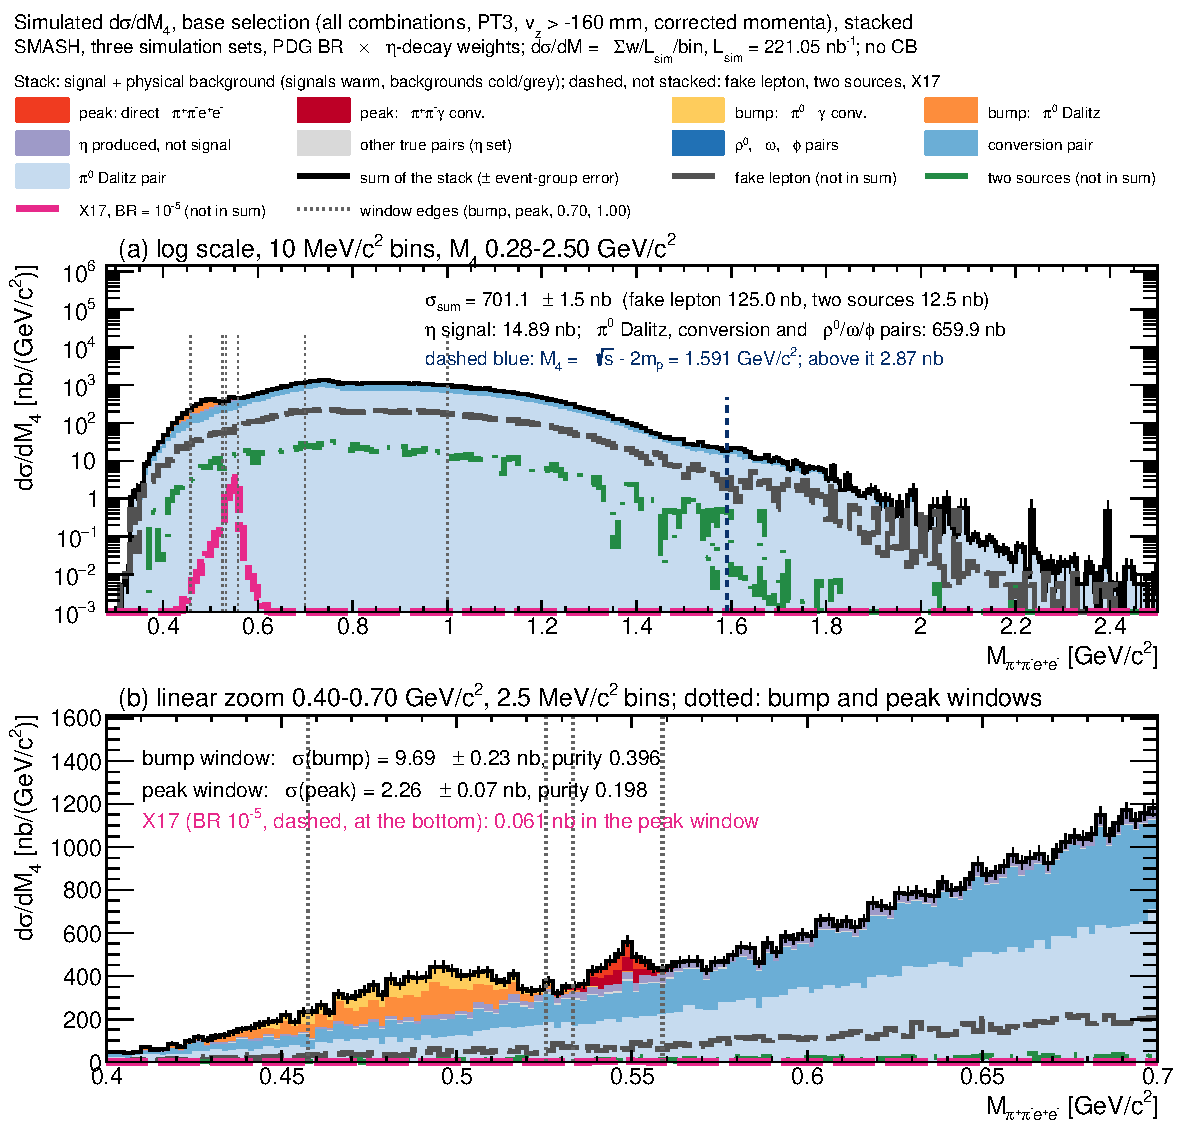
\includegraphics[width=0.62\textwidth]{figs/s5_spec_full_pre_short.pdf}
\caption{\textbf{What it shows: the $\eta$ peak and bump sit on a large background: over the whole range it is 46 times the
signal, inside the windows about 1.5 times (bump) and 4 times (peak) the signal.}
Simulated $d\sigma/d\Mfour$, stacked by component: $\eta$ signal channels in warm colours, background groups in cold
colours or grey. Dashed, not stacked: fake leptons, leptons from two sources and X17 at $\mathrm{BR}=10^{-5}$. (a) Log
scale over the full range; thin vertical lines: edges of the bump and peak windows and of the mass regions 0.5587--0.70,
0.70--1.00 and above 1.00\,\GeVcc of the tables of the full report; dashed blue: the largest \Mfour of p+p $\to pp\ppee$,
$\sqrt{s}-2m_p=1.591$\,\GeVcc (computed with the 4530\,MeV of the data kinematics; 1.583\,\GeVcc at the 4500\,MeV of
SMASH); the 2.87\,nb above it are mostly misidentified tracks. (b) Linear zoom with the bump and peak windows (dotted).
\sel \simonly; \basesel; no further cut; \simwin.
\infig $M_4=\Mfour$; $v_z$ = event-vertex $z$; $\Sigma w/L_{\mathrm{sim}}$ = weighted counts per simulated luminosity
$L_{\mathrm{sim}}$; event-group error = statistical error with all counts of one event taken together; purity = $S/(S+B)$ in the
window.}
\label{fig:spec}
\end{figure}

\begin{figure}[!htbp]
\centering
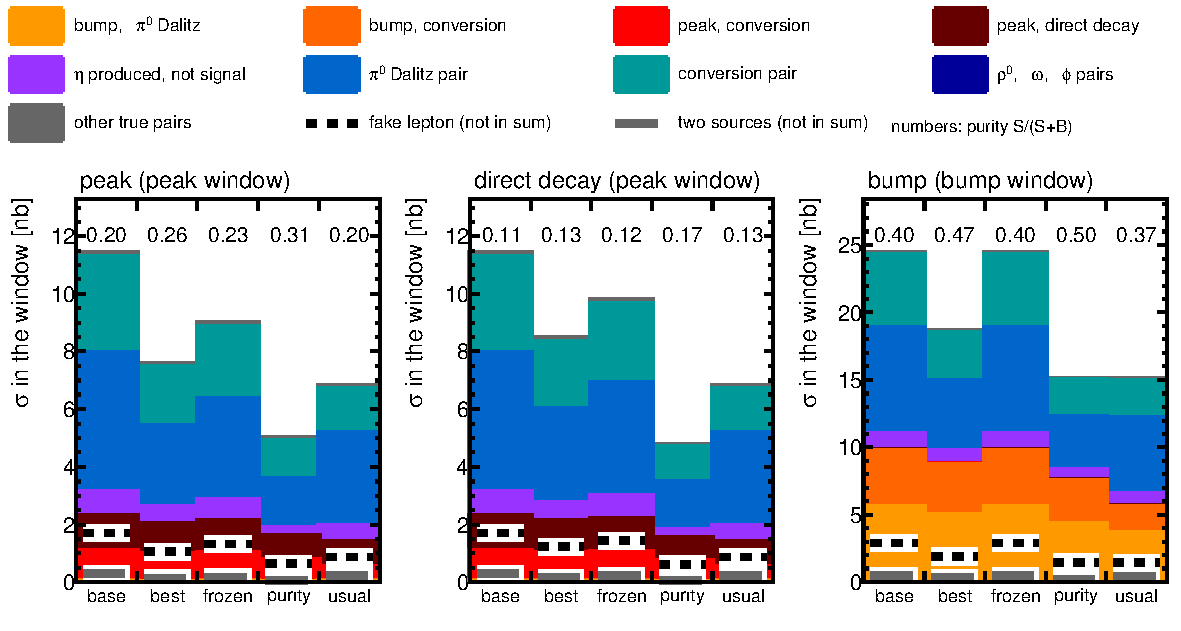
\includegraphics[width=0.78\textwidth]{figs/s5_opt_eta_composition_plain.pdf}
\caption{\textbf{What it shows: the usual $\eta$ cuts remove signal and background alike, so the purity of the windows
does not rise.} Content of the peak window (left: both peak channels; middle: direct decay only) and of the bump window
(right), $\sigma$ in nb, stacked by component (signal at the bottom, warm colours), for five selections. Fake leptons
(black-and-white dashes) and leptons from two sources (grey marks) are not in the stack. Numbers above the bars: purity,
rounded; from the first to the last bar it goes $0.198\to0.202$ (peak) and $0.396\to0.371$ (bump); the frozen peak selection
has 0.23.
\sel \simonly; \basesel; \simwin; then per bar: (1)~no further cut; (2)~the best cut combination of the scan
(peak: $0.32<\Mpipi<0.48$\,\GeVcc, angle in the $\eta$ rest frame above $160^\circ$, both pion tracks within 40\,mm of the
event vertex along the beam, missing mass of \ppee below 2.85\,\GeVcc; direct decay: $0.30<\Mpipi<0.53$\,\GeVcc, angle in
the $\eta$ rest frame above $150^\circ$, pion tracks within 40\,mm, missing mass below 2.85\,\GeVcc; bump: angle between
\pipi and \ee in the laboratory below $70^\circ$, $0.30<\Mpipi<0.41$\,\GeVcc, pion tracks within 40\,mm); (3)~the frozen
selection (peak: pion tracks within 40\,mm and missing mass below 2.85\,\GeVcc; direct decay: pion tracks within 40\,mm;
bump: no further cut); (4)~the highest purity within 5\,\% of the best $F$ with at most three cuts (peak:
$\Mpipi>0.32$\,\GeVcc, pion tracks within 40\,mm, missing mass below 2.7\,\GeVcc; direct decay: laboratory angle below
$40^\circ$, pion tracks within 40\,mm, missing mass below 2.7\,\GeVcc; bump: laboratory angle below $40^\circ$,
$\Mpipi>0.32$\,\GeVcc, pion tracks within 40\,mm); (5)~the usual $\eta$ cuts (\usualcuts).
\infig the bars base, best, frozen, purity, usual are (1)--(5).}
\label{fig:res_cuts}
\end{figure}

\begin{figure}[!htbp]
\centering
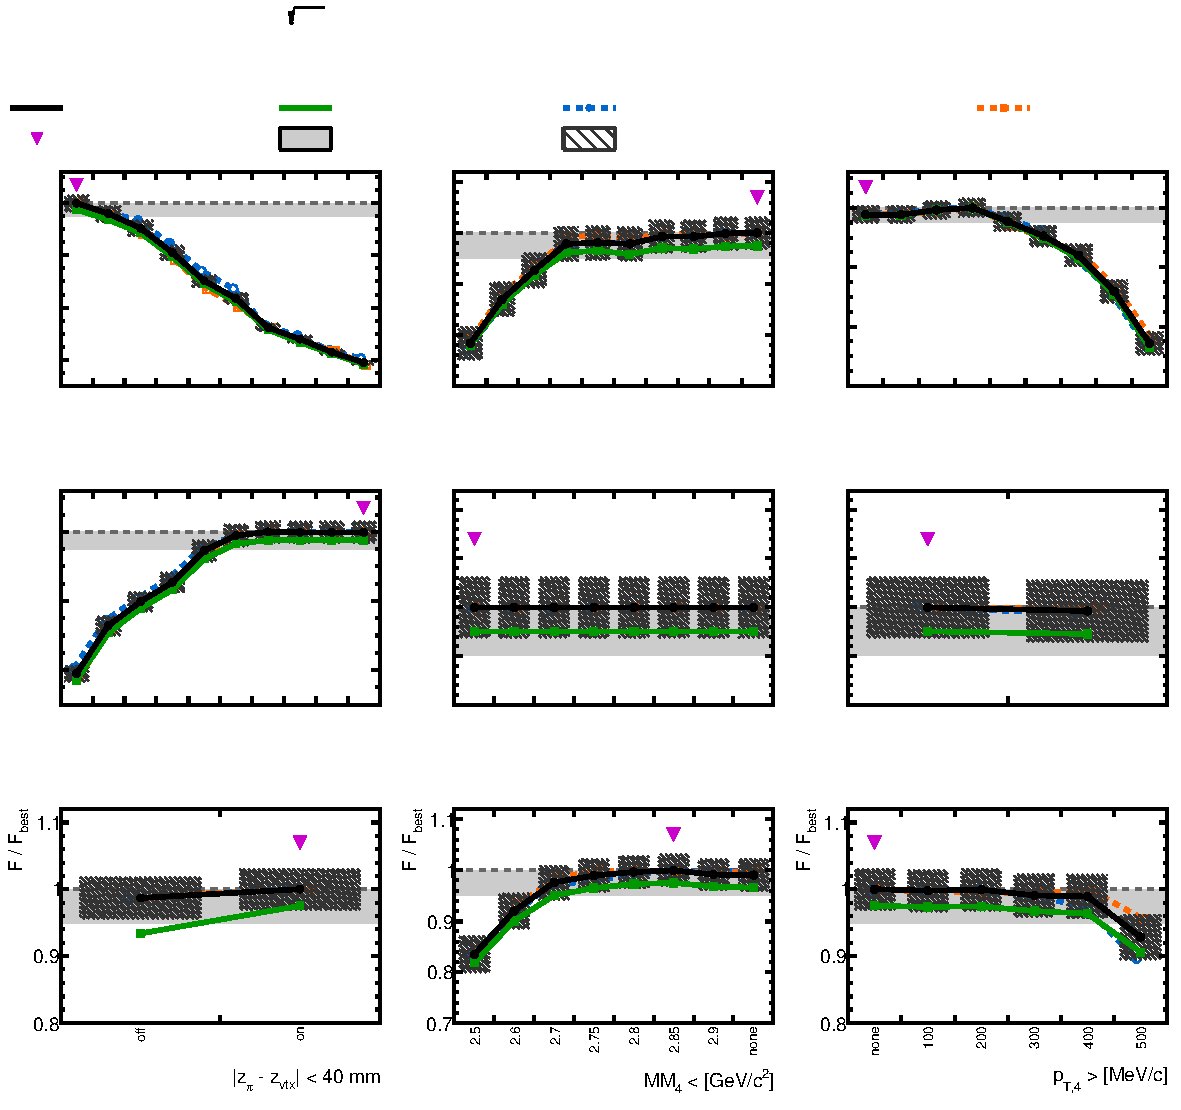
\includegraphics[width=0.84\textwidth,trim=0 0 0 380,clip]{figs/s5_opt_eta_profile_peak_cnt_short.pdf}
\caption{\textbf{What it shows: the optimum is flat; the frozen peak cuts (triangles; only their horizontal position counts,
they are drawn above the curves) sit on its plateau.} $F/F_{\mathrm{best}}$
of the peak against the cut on the pion tracks (off/on), on the missing mass of \ppee and on the transverse momentum of
\ppee (bottom row of the nine-variable profile of the full report; $F_{\mathrm{best}}=56.2$). Black: the best $F$ over all
other cut variables at a fixed value (the nine scanned variables: \ee opening angle above 10 values, laboratory angle
between \pipi and \ee below 10 values, \Mpipi above 9 and below 10 values, the same angle in the $\eta$ rest frame above
8 values, both pions used in the vertex fit off/on, the pion-track cut off/on, missing mass below 8 values and $p_T$ of
\ppee above 6 values; 13.8 million combinations); dashed: the same in the two halves of the sample; hatched: $\pm1\sigma$ statistical
error; green: slice through the frozen selection; grey band: within 5\,\% of the best $F$; triangle: frozen value. The
frozen peak selection gains 5\,\% in $F$ over the base selection.
\sel \simonly; \basesel; $S$ = both peak channels and $B$ = all other signal and physical-background counts in the peak
window $0.5333\le\Mfour<0.5587$\,\GeVcc (simulation mass scale), at 6080.5\,\nbinv; frozen point: both pion tracks within
40\,mm of the event vertex along the beam and missing mass of \ppee below 2.85\,\GeVcc, no other cut.
\infig $|z_\pi-z_{\mathrm{vtx}}|<40$\,mm = both pion tracks within 40\,mm of the event vertex along the beam;
MM$_4$ = missing mass of \ppee; $p_{T,4}$ = transverse momentum of \ppee; none, off = no cut. $S$ and $B$ at 6080.5\,\nbinv.}
\label{fig:res_frozen}
\end{figure}

\begin{figure}[!htbp]
\centering
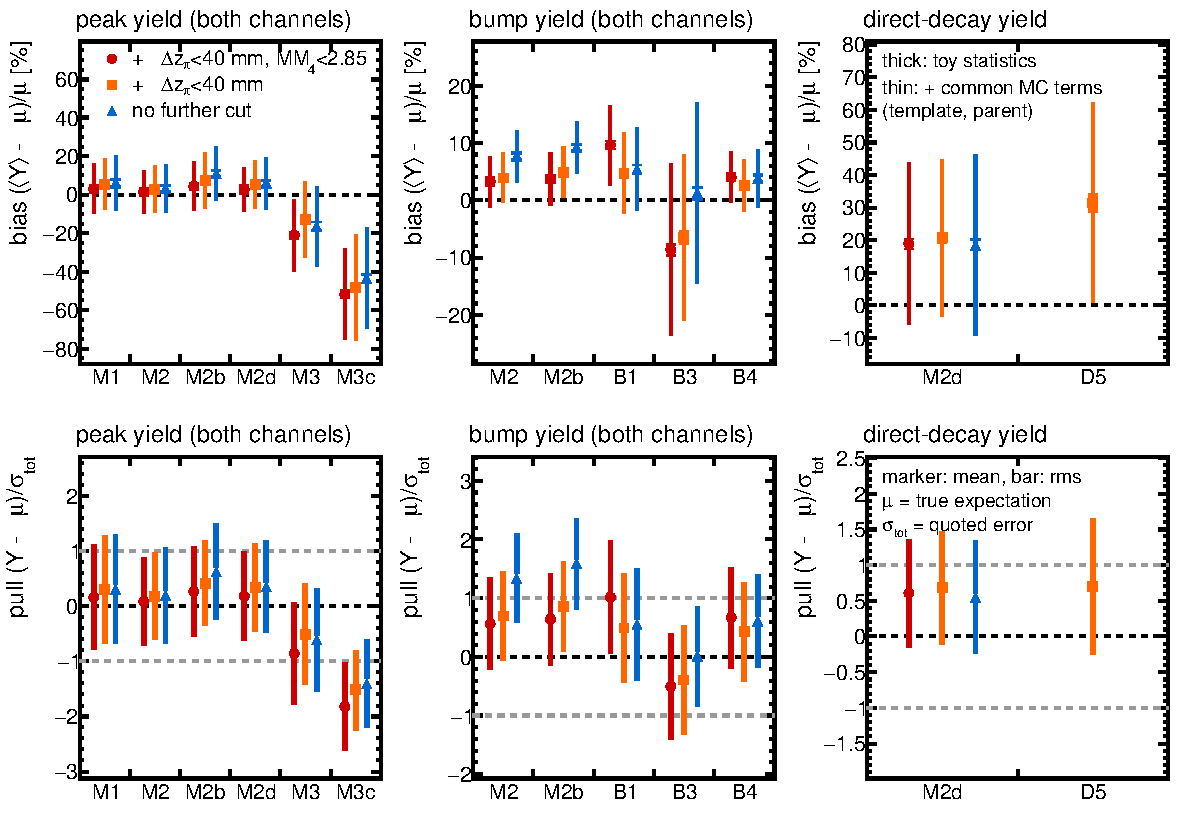
\includegraphics[width=0.66\textwidth]{figs/s5_blind_eval_eta_bias_plain.pdf}
\caption{\textbf{What it shows: in this test template and Gaussian fits recover the peak; linear side bands lose it.}
Blind test of the $\eta$ yields: 200 pseudo-data sets of 110.5\,\nbinv from one half of the simulated events, templates
from the other half. Top: relative bias per method and selection (thick bars: statistics of the pseudo-data, thin bars:
including the common simulation error). Bottom: pull, marker = mean, bar = rms. Plain linear side bands (M3) lose
13--46\,\% over all tests; with the simulated curvature (M3c) they lose even more ($-44$ to $-52$\,\%), because that curvature
is itself noisy in the simulation. The fits look good here partly because the template noise of this split is not that of a
real analysis (Fig.~\ref{fig:stress}).
\sel \simonly; \basesel; red: plus both pion tracks within 40\,mm of the event vertex along the beam and missing mass of
\ppee below 2.85\,\GeVcc (frozen peak selection); orange: plus the pion-track cut only (frozen direct-decay selection);
blue: no further cut (frozen bump selection); \simwin. Pseudo-data: \Mfour 0.30--1.20\,\GeVcc.
\infig methods on the horizontal axis: M1 = Gaussian (fixed at 0.5460\,\GeVcc, width 6.7\,\MeVcc) + second-order polynomial
fitted in 0.526--0.614\,\GeVcc, calibrated (its content converted to the peak-window yield with the simulated peak shape);
M2 = template fit in 0.400--0.700\,\GeVcc; M2b = the same with the other $\eta$ decays free;
M2d = template fit of the direct decay with the conversion peak constrained; M3 = linear side bands 0.5255--0.5333 and
0.5587--0.5665\,\GeVcc, M3c = the same with the simulated curvature; B1 = parametric fit of the bump in 0.400--0.620\,\GeVcc
(asymmetric Gaussian bump + $\eta$ Gaussian + second-order polynomial); B3 = step at the kinematic edge of the bump; B4 = side band 0.5665--0.70\,\GeVcc with the simulated
background shape; D5 = direct decays from a split at $\Mee=10$\,\MeVcc. $\mu$ = true content of the pseudo-data;
$\sigma_{\mathrm{tot}}$ = quoted error; MC = simulation statistics.}
\label{fig:bias}
\end{figure}

\begin{figure}[!htbp]
\centering
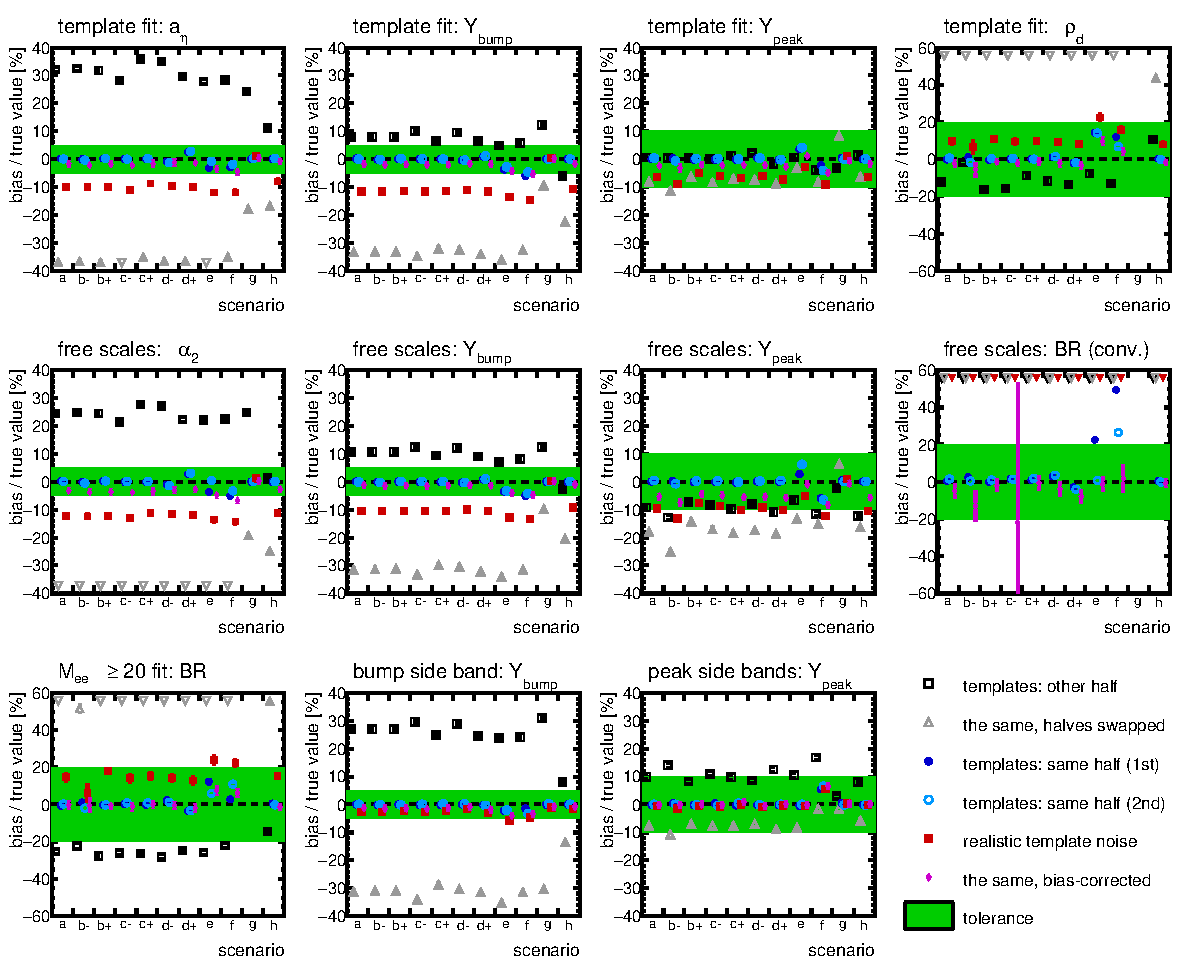
\includegraphics[width=0.74\textwidth]{figs_all/wp4_V1_plain.pdf}
\caption{\textbf{What it shows: with the template noise of a real analysis (red squares) the template fits of the $\eta$ scale
and of the yields come out low ($\eta$ scale $-10.1$\,\%, bump yield $-11.6$\,\%, peak yield $-6.6$\,\%), while the
direct-decay scale and the branching ratios come out high (for example $+14.8$\,\% for the branching ratio from the fit at
$\Mee\ge20$\,\MeVcc); the side bands (bottom row, middle and right) are not biased.} Finding of Part~III
(\code{report_all.pdf}): relative bias of each estimated quantity in the truth scenarios (a)--(h) of its stress test, 500
pseudo-data sets per point at the luminosity of the analysed runs, 6079.2\,\nbinv. The truth is the smoothed simulated
background plus the simulated $\eta$ channels plus a CB built from the like-sign pairs of the \emph{data}, so this is not a
simulation-only figure. Open squares: truth from one half of the simulation, templates from the other (the kind of split of the
blind test of this part, Fig.~\ref{fig:bias}); grey triangles: the halves swapped. Here the two halves of the smoothed
background differ by 5--10\,\% per 50\,\MeVcc band of \Mfour, and this single difference moves the $\eta$ scale by $+32$\,\% or
$-37$\,\%: such a split has four times the template noise of the real analysis, and Part~III does not use it as its test.
Circles: truth and templates from the same half (the methods close exactly); red squares: truth from the full sample,
templates from bootstrap copies of the simulation (exactly the template noise of the real analysis); magenta: red squares with
a bias correction. Green band: tolerance (5\,\% for the $\eta$ scale and the bump yield, 10\,\% for the peak yield, 20\,\% for
the direct-decay scale and the branching ratios).
\sel as in Part~III, on the data mass scale: \basesel; both pion tracks used in the event-vertex fit; CB $=2\sqrt{N_{++}N_{--}}$ from the
like-sign data ($\pi^+\pi^-e^+e^+$, $\pi^+\pi^-e^-e^-$) with the same cuts. Template fits: \Mfour 0.40--0.70\,\GeVcc in the
five \Mpipi slices below 0.34, 0.34--0.37, 0.37--0.39, 0.39--0.43 and above 0.43\,\GeVcc, \Mee of 10\,\MeVcc or more (bottom
left: 20\,\MeVcc or more). Bump side band: bump window 0.4550--0.5225\,\GeVcc, background carried down from
0.575--0.70\,\GeVcc ($\Mee\ge10$\,\MeVcc) with the simulated shape. Peak side bands: peak window 0.53364--0.55416\,\GeVcc,
side bands 0.5250--0.5336 and 0.5542--0.5628\,\GeVcc.
\infig template fit = the fit of the five \Mpipi slices with one $\eta$ scale; free scales = the same with a free scale per
$\eta$ channel; $a_\eta$ = $\eta$ scale relative to SMASH; $Y_{\mathrm{bump}}$, $Y_{\mathrm{peak}}$ = bump and peak yields;
$\rho_d$ = direct-decay scale; $\alpha_2$ = scale of the bump with a \piz Dalitz pair; BR (conv.) = $\mathrm{BR}(\eta\to\ppee)$
from the converted photons; $\Mee\ge20$ fit: BR = the same from the template fit at $\Mee\ge20$\,\MeVcc. Scenarios: (a) background $\times1.35$ with a linear tilt $-0.15$ and $\eta$ scale 0.4; (b$-$, b$+$) direct-decay scale 0.5,
1.5; (c$-$, c$+$) conversion scale of the signal 0.8, 1.2; (d$-$, d$+$) scale of the other $\eta$ decays 0.5, 1.5; (e) background
with pions from $\omega$ or $\rho^0$ $\times0.3$, the rest $\times1.6$; (f) simulated mass scale $+0.0009$ and resolution
$\times0.89$; (g) no $\eta$; (h) $\eta$ scale 1.}
\label{fig:stress}
\end{figure}

\begin{figure}[!htbp]
\centering
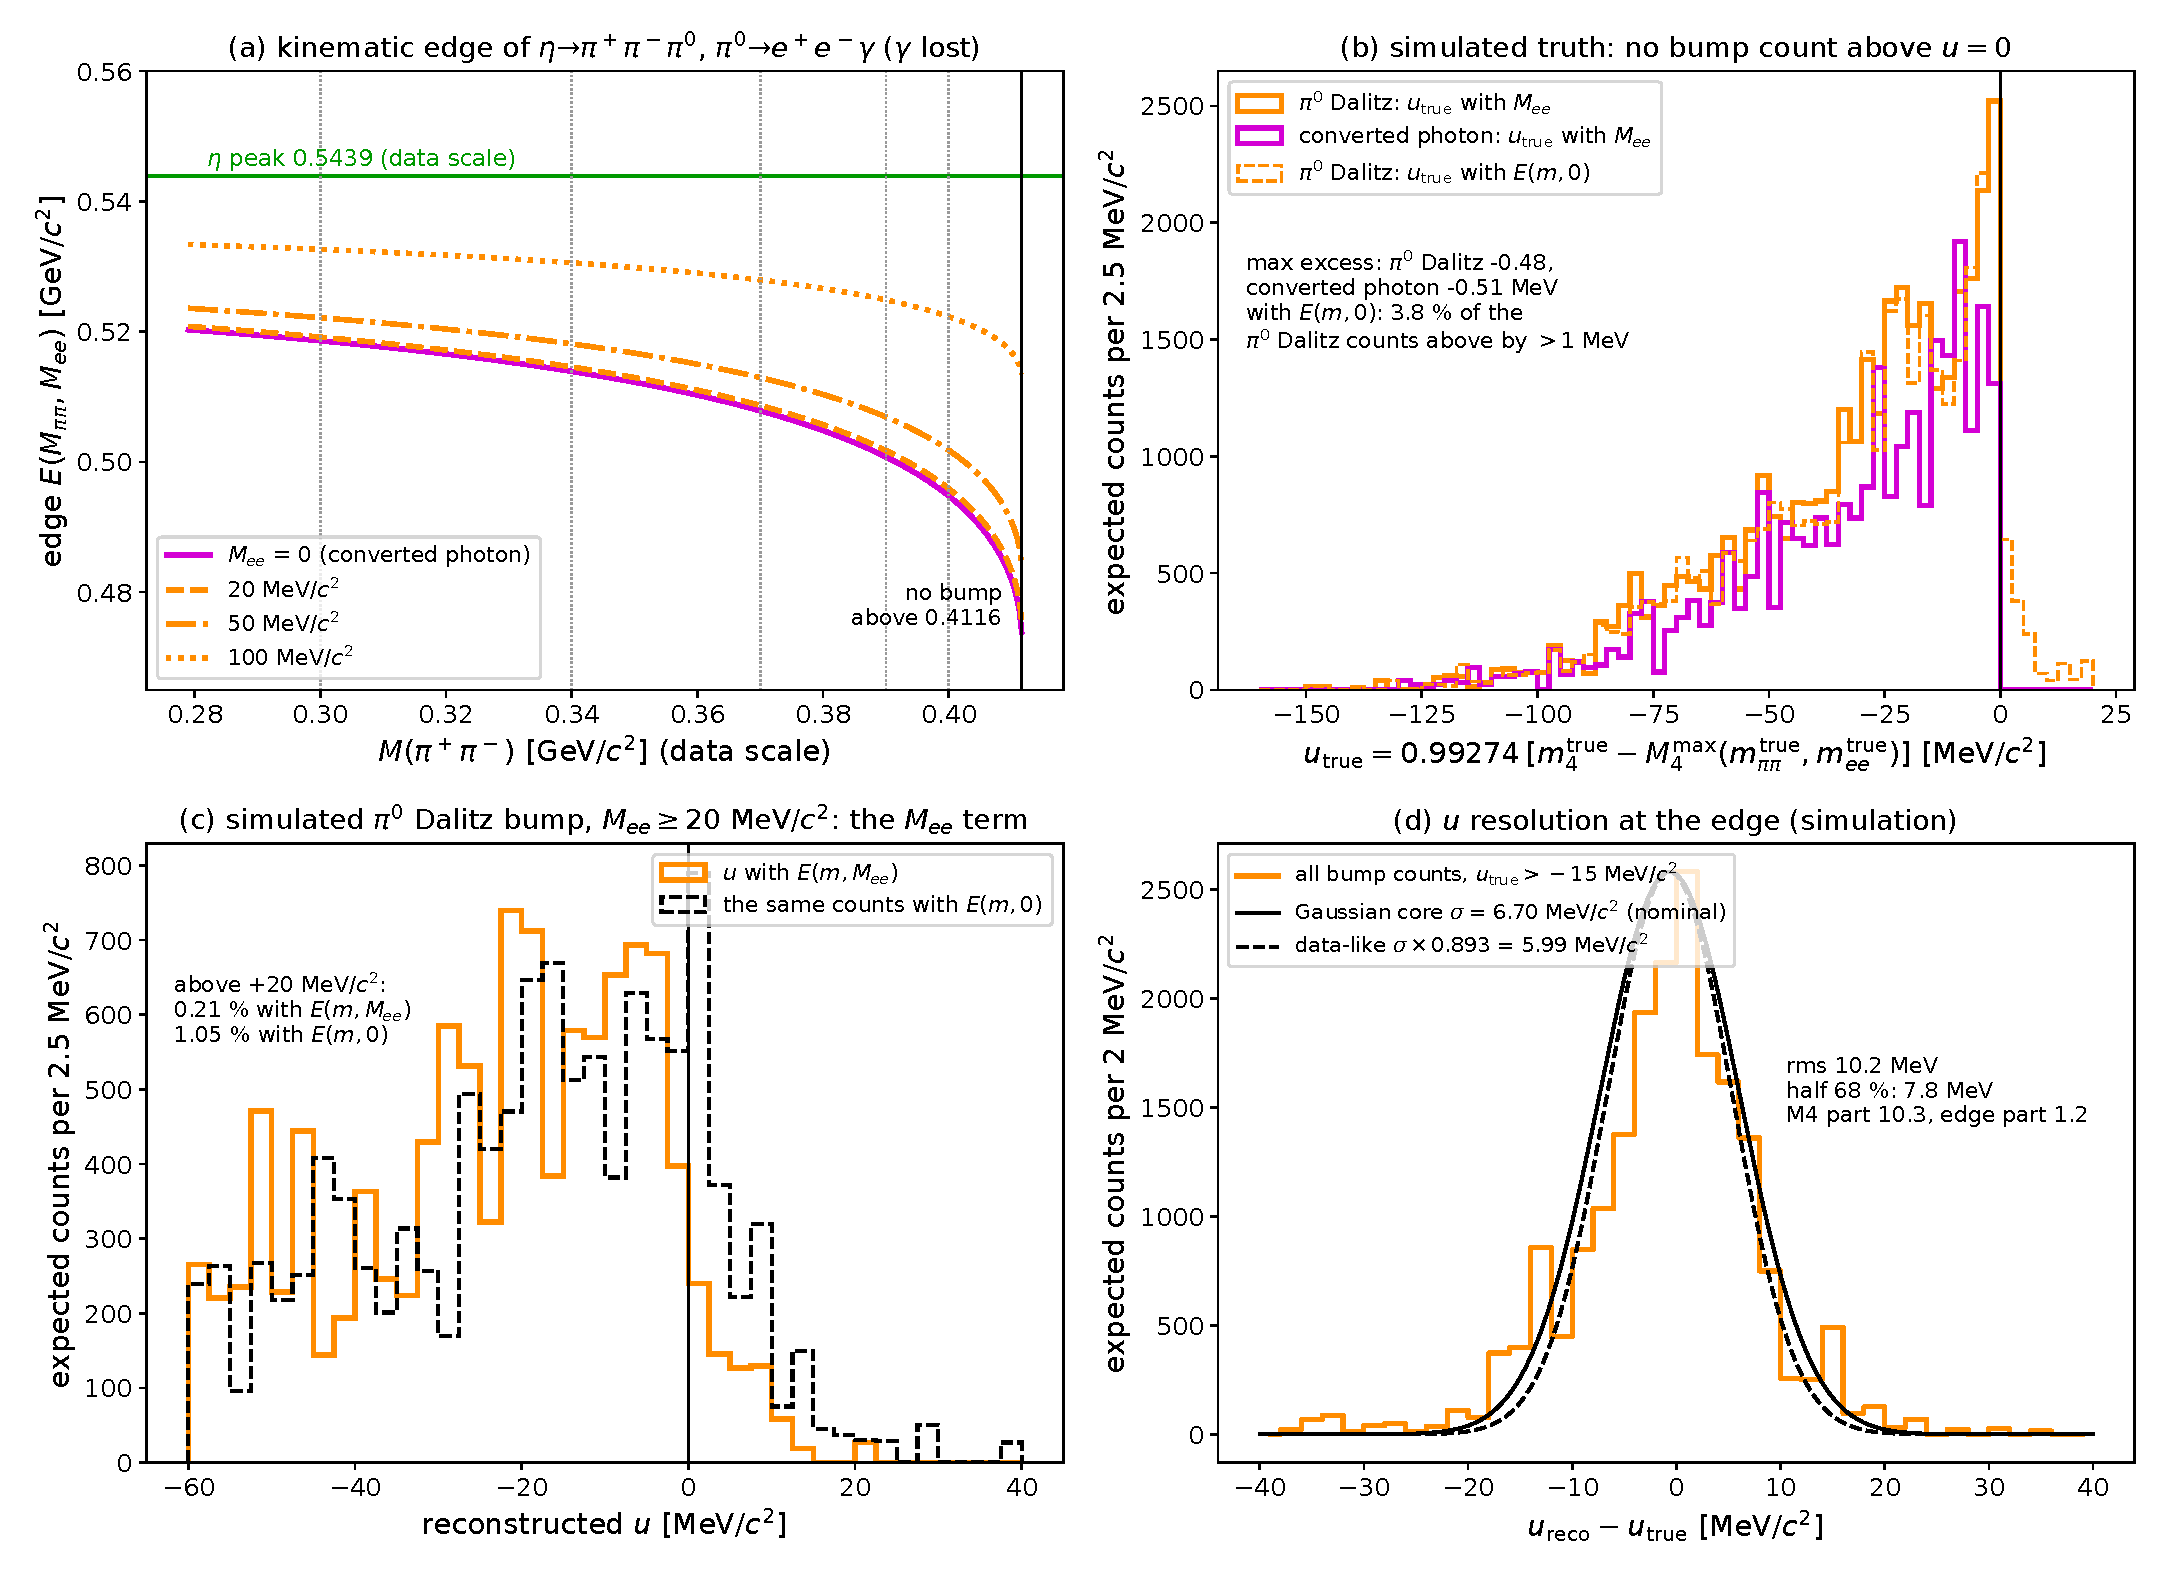
\includegraphics[width=0.70\textwidth]{figs_all/edgeu_kinematics_cnt_plain.pdf}
\caption{\textbf{What it shows: once the edge of the bump is computed with both \Mpipi and \Mee, no simulated bump count
lies above it, so in the distance to it, $u$, all bump counts end at $u=0$; the reconstructed $u$ is smeared with a Gaussian
core of 6.7\,\MeVcc (rms 10.2\,\MeVcc).} Finding of Part~III; simulation only. (a) The edge $E(\Mpipi,\Mee)$ for $\Mee=0$,
20, 50 and 100\,\MeVcc; green: the $\eta$ peak; no bump above $\Mpipi=0.4116$\,\GeVcc; dotted vertical lines: the \Mpipi
slices 0.30--0.34, 0.34--0.37, 0.37--0.39, 0.39--0.40\,\GeVcc of the edge fits. (b) True $u$ of the bump with a \piz Dalitz
pair (orange) and with a converted photon (magenta); dashed: the Dalitz pairs with the edge taken at $\Mee=0$, which puts
counts above $u=0$. (c) Reconstructed $u$ of the bump with a \piz Dalitz pair and $\Mee\ge20$\,\MeVcc, with and without the
\Mee term. (d) Reconstructed minus true $u$ for all bump counts with a true $u$ above $-15$\,\MeVcc (near the edge): Gaussian
core 6.7\,\MeVcc, rms 10.2\,\MeVcc, half-width of the central 68\,\% 7.8\,\MeVcc (dashed: core $\times0.893$, the width
favoured by the data peak).
\sel SMASH simulation only (no combinatorial background), main $\eta$-decay physics weights, expected counts at the
6079.2\,\nbinv of the analysed runs; \basesel; both pion tracks used in the event-vertex fit; simulated masses moved to the
data mass scale ($\Mfour\times0.99615$, $\Mpipi\times0.9952$); $u$ exists for \Mee below 135\,\MeVcc (the \piz mass).
\infig $E(m,M_{ee})$ = edge at $\Mpipi=m$ with the \Mee term, $E(m,0)$ = without it; $u_{\mathrm{true}}$ = true distance to the
edge (0.99274 = data mass scale of the $\eta$ peak); $M_4$, $M_4^{\max}$ = \Mfour and its largest value for the bump.}
\label{fig:res_edgeu}
\end{figure}

\begin{figure}[!htbp]
\centering
\begin{minipage}[b]{0.40\textwidth}\centering
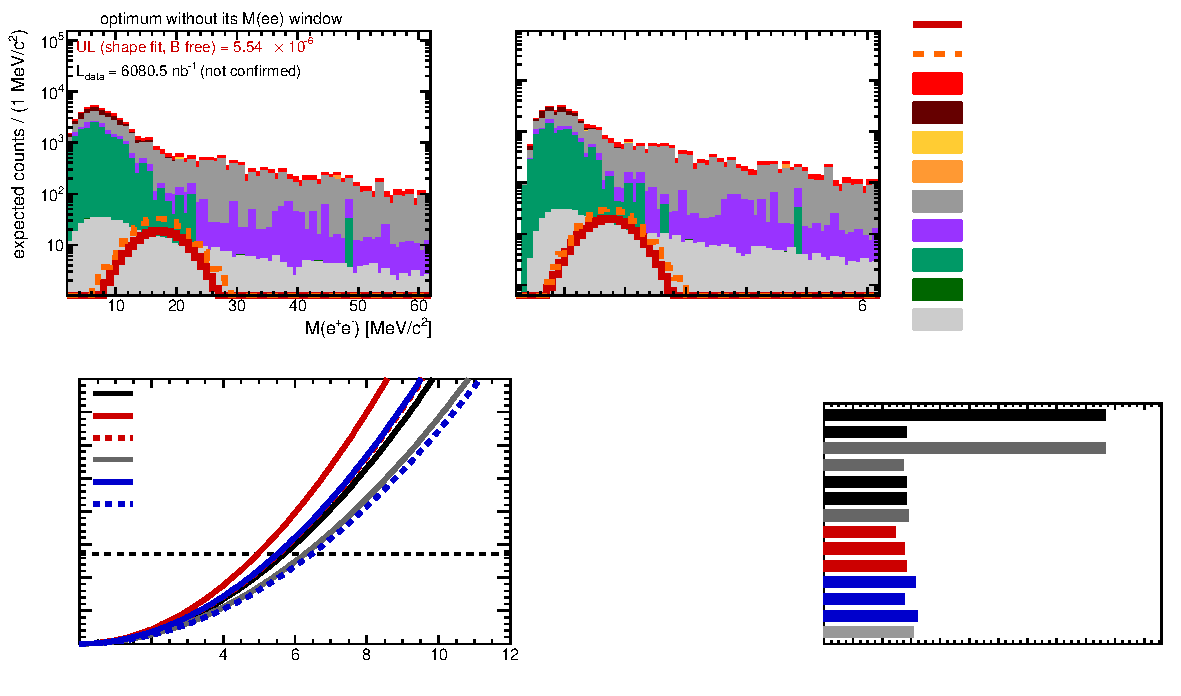
\includegraphics[width=\textwidth,trim=0 168 355 0,clip]{figs/s5_opt_x17_shape_cnt_shortA.pdf}
\end{minipage}\hfill
\begin{minipage}[b]{0.56\textwidth}\centering
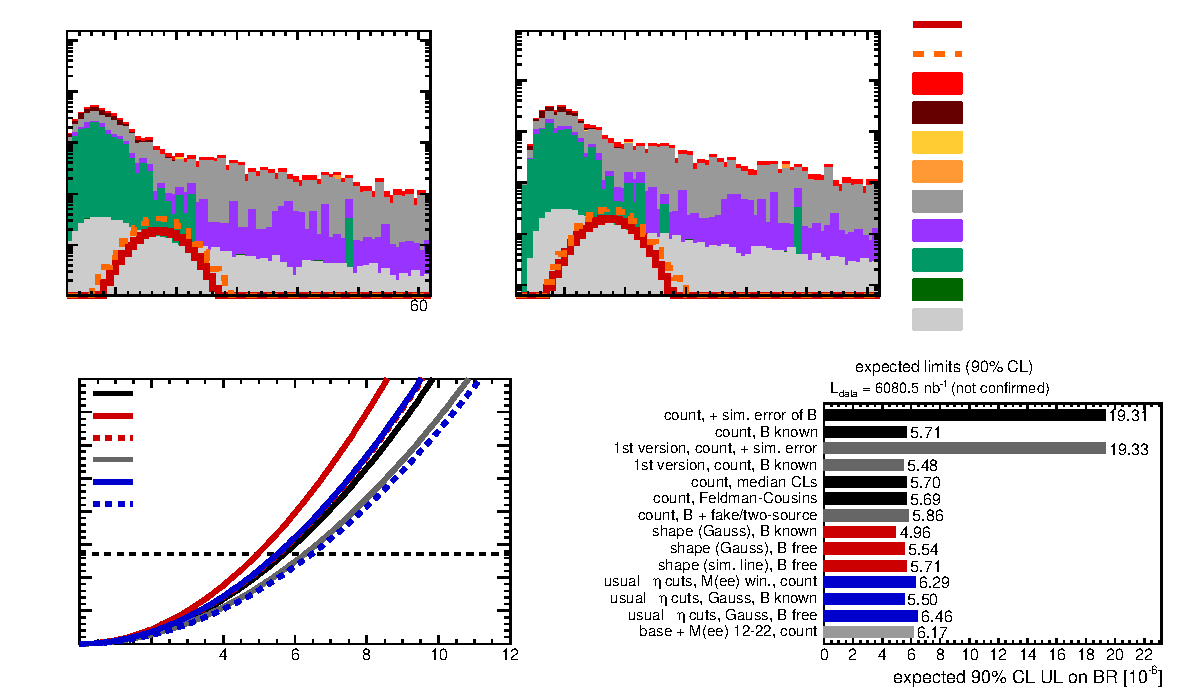
\includegraphics[width=\textwidth,trim=280 0 0 166,clip]{figs/s5_opt_x17_shape_cnt_shortB.pdf}
\end{minipage}
\caption{\textbf{What it shows: the X17 limit is set by the simulation error of the background.} Expected counts at
\Ldata (not confirmed). Left: \Mee in the peak window, X17 selection without its \Mee window; stacked background (dark grey:
\piz Dalitz pairs, green: conversion pairs, purple: $\eta$ without signal, red: direct decay, light grey: other), X17 at its
expected limit (dark red Gaussian) and the simulated X17 at $\mathrm{BR}=10^{-5}$ (orange dashed). Right: expected 90\,\% CL
limits for several selections and methods, in units of $10^{-6}$ (background normalisation known unless stated); the top
two bars are the $1.9\times10^{-5}$ with the simulation error of the background and the $5.7\times10^{-6}$ with the background
known exactly. Shape fits use \Mee 2--62\,\MeVcc in 1\,\MeVcc bins.
\sel \simonly; \basesel; both pion tracks used in the event-vertex fit; peak window $0.5333\le\Mfour<0.5587$\,\GeVcc
(simulation mass scale); $15.5\le\Mee<24.5$\,\MeVcc (left: this \Mee window left out).
\infig count = counting in the window; B known / B free = background normalisation fixed / free; + sim.\ error of B = with
the simulation error of the background; 1st version = the first version of the X17 selection ($13.0\le\Mee<26.5$\,\MeVcc,
$0.5330\le\Mfour<0.5555$\,\GeVcc); usual $\eta$ cuts = the base selection with the usual $\eta$ cuts (\usualcuts) in the
peak window; M(ee) win.\ = with the X17 \Mee window; base + M(ee) 12--22 = the base selection with $12\le\Mee<22$\,\MeVcc;
shape (Gauss) / (sim.\ line) = fit of the \Mee shape with a Gaussian / with the simulated X17 line; B + fake/two-source =
background with fake leptons and leptons from two sources; UL = upper limit; median CLs, Feldman--Cousins = other limit
methods.}
\label{fig:res_x17}
\end{figure}

\begin{figure}[!htbp]
\centering
\begin{minipage}[b]{0.50\textwidth}\centering
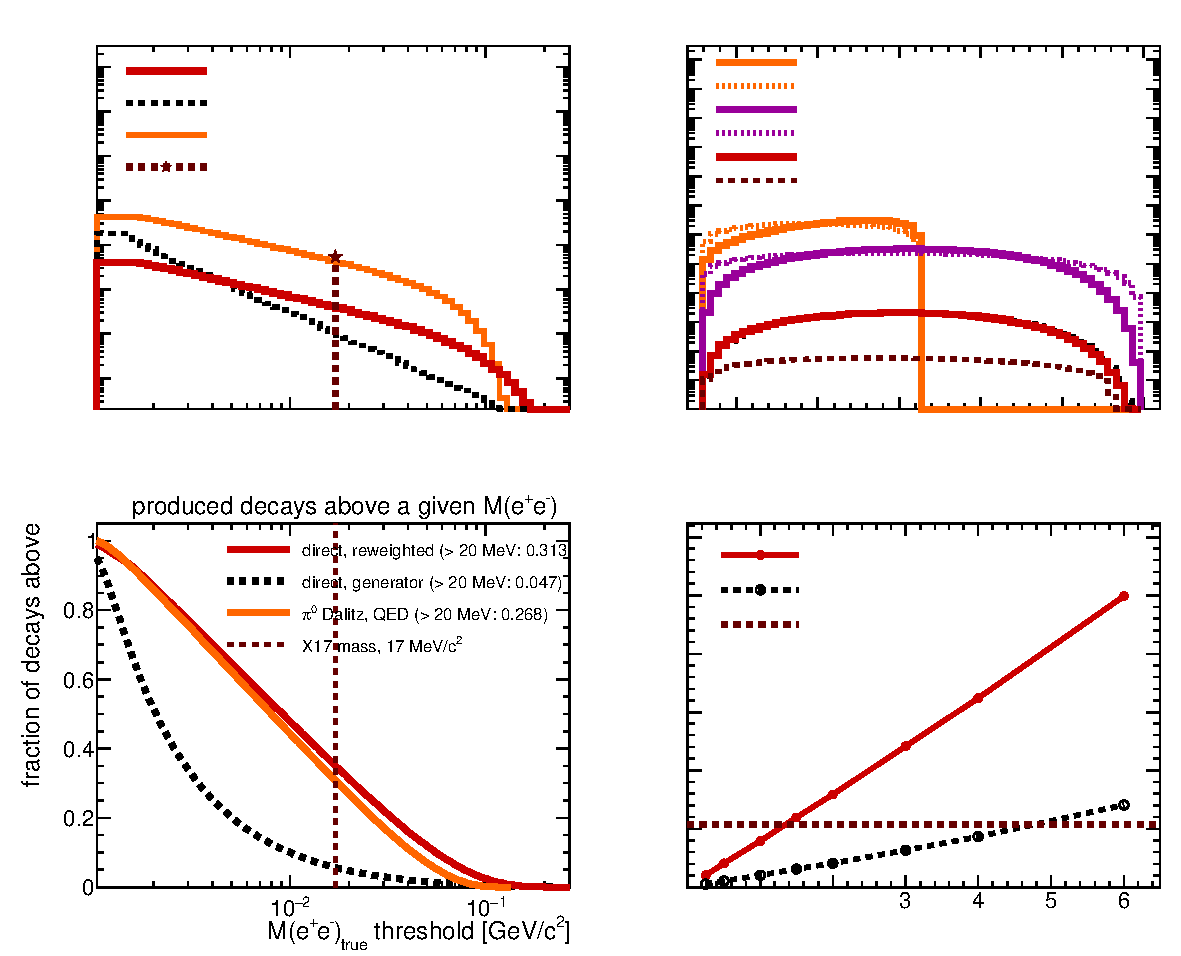
\includegraphics[width=\textwidth,trim=0 0 284 231,clip]{figs/s5_acc_gen_short.pdf}
\end{minipage}\hfill
\begin{minipage}[b]{0.40\textwidth}\centering
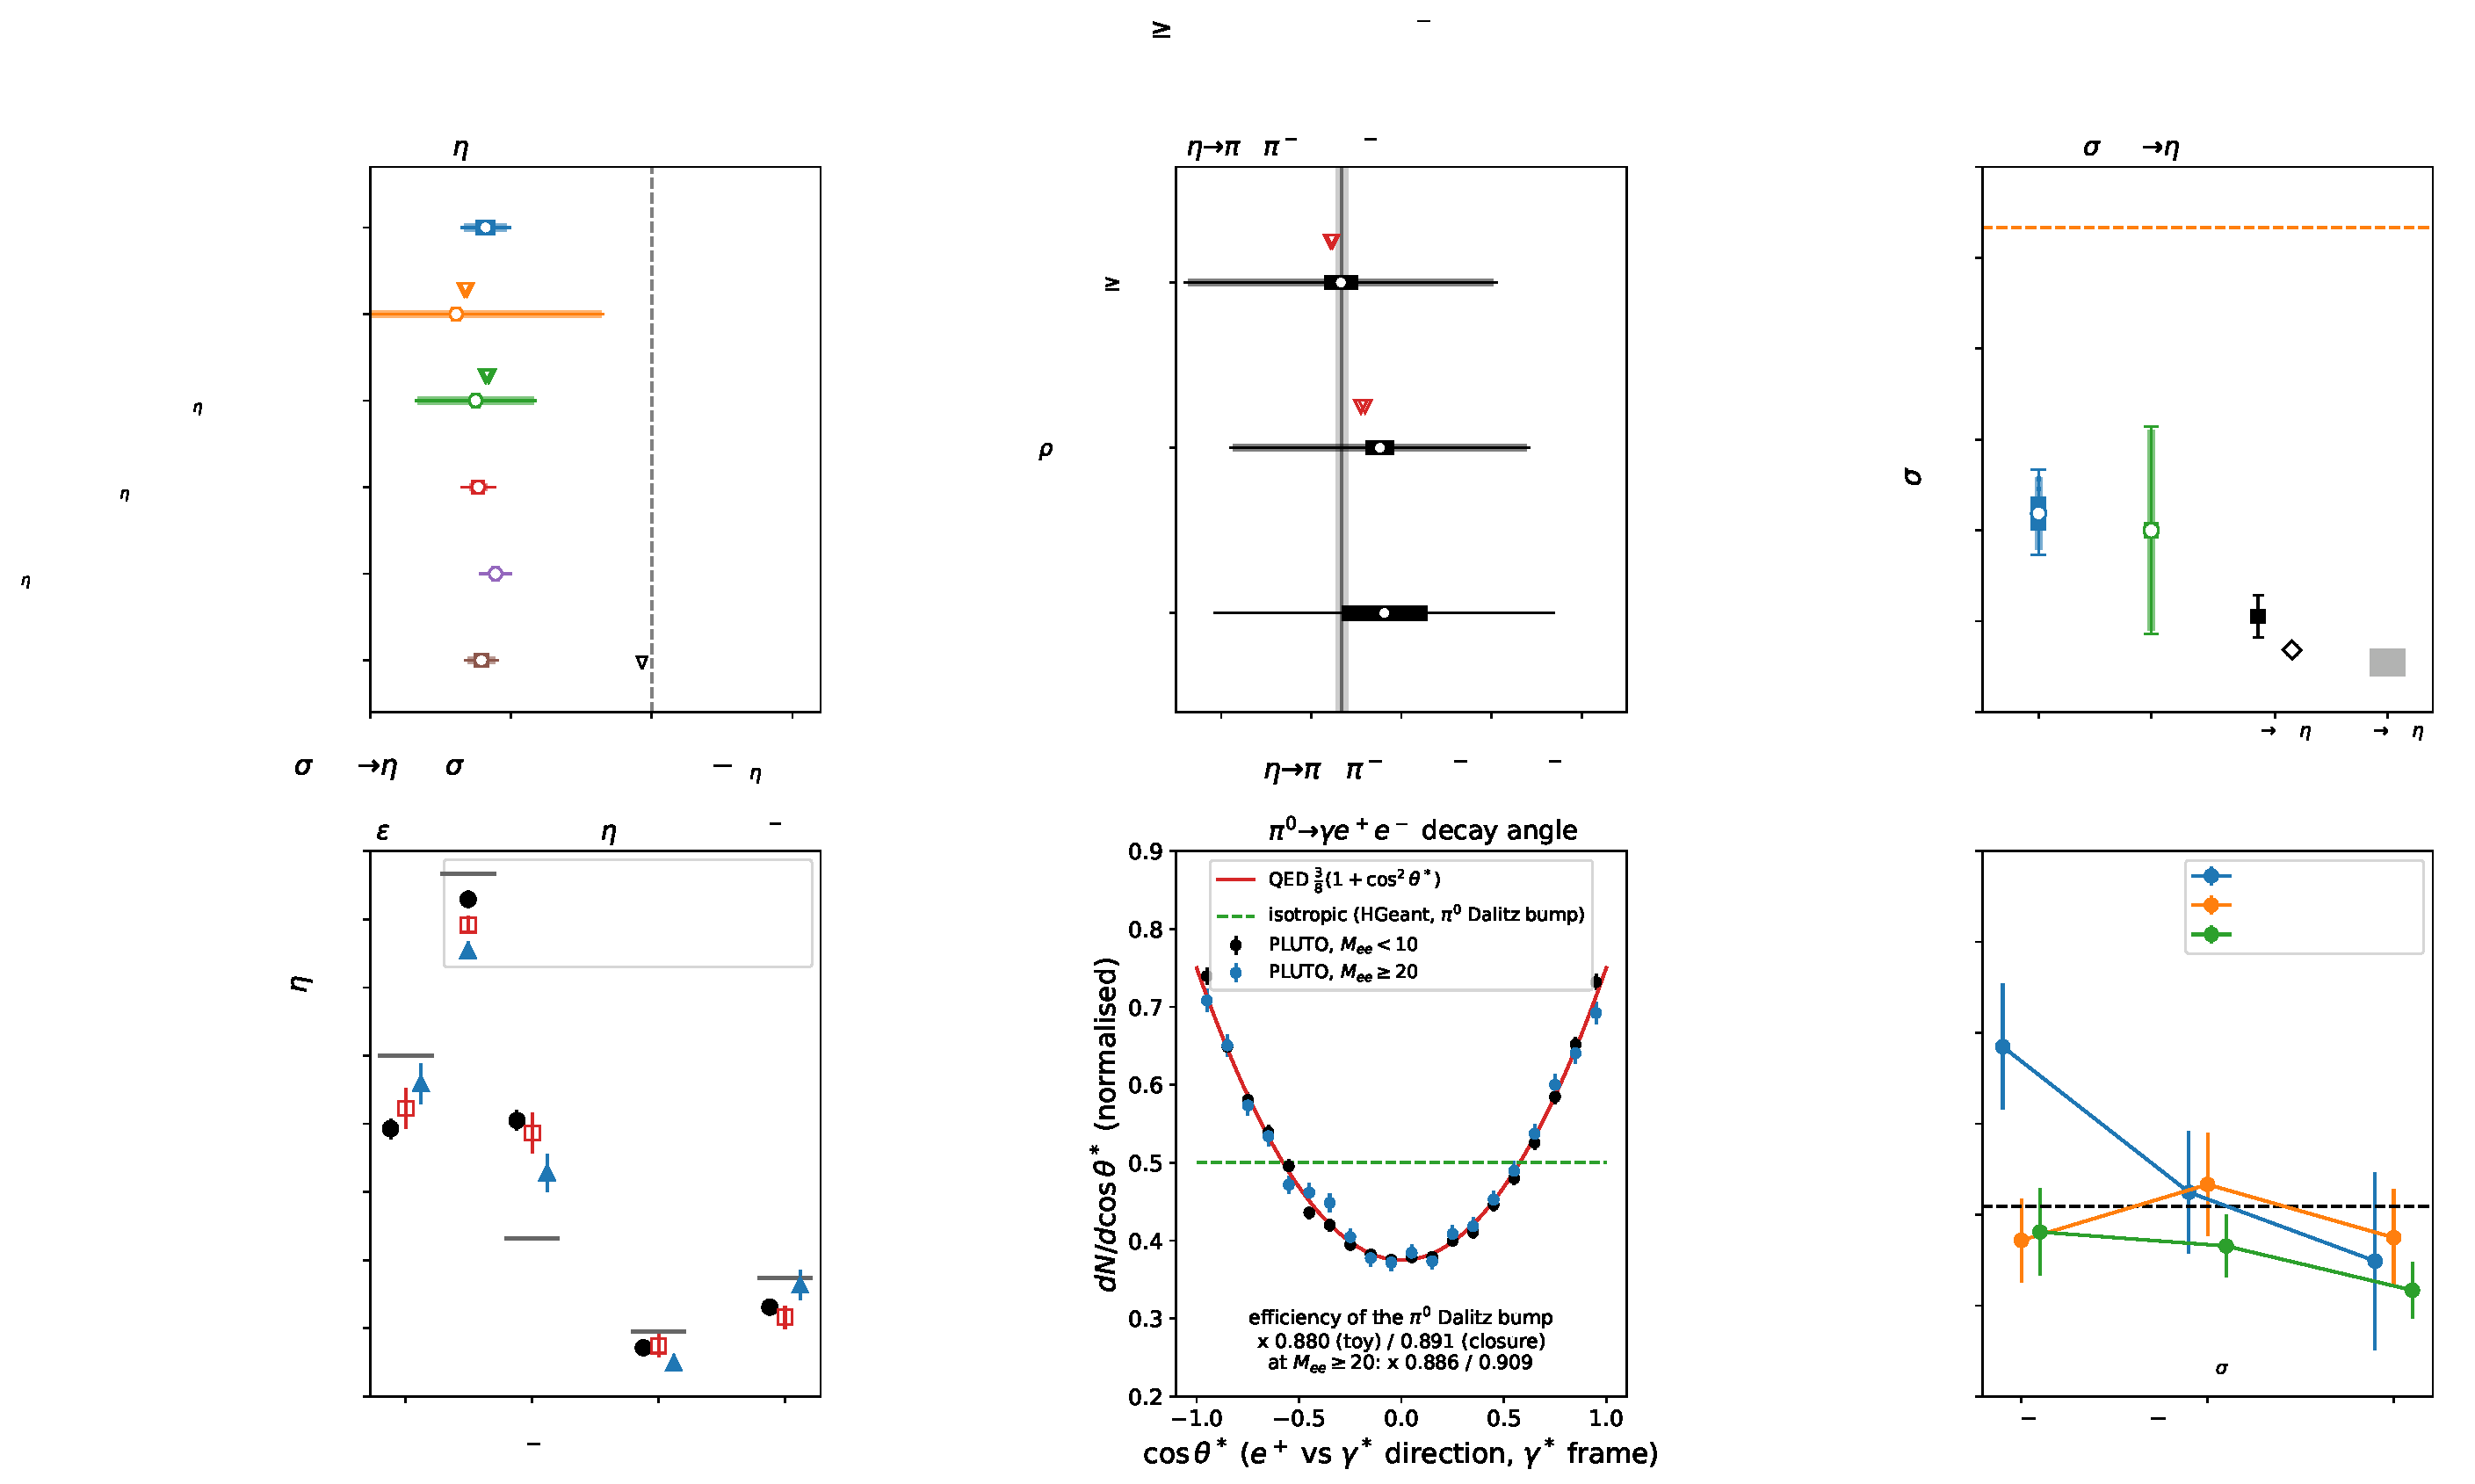
\includegraphics[width=\textwidth,trim=594 5 447 437,clip]{figs_all/wp8_P1_shortI.pdf}
\end{minipage}
\caption{\textbf{What it shows: two wrong decay distributions of the simulation, one corrected here (left), one found with
Part~III (right).}
Left: fraction of the produced $\eta\to\ppee$ decays above a given \Mee. The generator (dotted black) has only 4.7\,\% of
the pairs above 20\,\MeVcc; reweighted to Kroll--Wada with form factors and decay angles (red, the main physics weights) it
has 31.3\,\% (Kroll--Wada with phase space only, not drawn, gives 28\,\%). Orange, for comparison: the analytic QED
(Kroll--Wada) distribution of the \piz Dalitz pair (26.8\,\% above 20\,\MeVcc); vertical line: the X17 mass. Right (Part~III,
\code{report_all.pdf}): decay angle of the virtual photon in $\piz\to\ee\gamma$. PLUTO (points) follows QED,
$1+\cos^2\theta^*$ (red line); HGeant, which decays the \piz of the standard set, decays it isotropically (green). So the
standard set accepts too many \piz Dalitz pairs: the lepton set (PLUTO) holds $0.891\pm0.003$ of the accepted prompt \piz
Dalitz pairs of the standard set, and reweighting the isotropic decays to QED in a pseudo-experiment gives 0.880 (the factors
printed in the panel); for the bump of this analysis the full simulation with a QED weight per count gives 0.864, i.e.\ the
simulated efficiency is about 16\,\% too high (Sect.~\ref{sec:corr}).
\sel no cut: all produced decays at generator level, before the detector (left: SMASH $\eta$ production; right: the \piz
Dalitz decays of PLUTO in the lepton set, 124\,k decays, $\Mee<10$\,\MeVcc and $\Mee\ge20$\,\MeVcc).
\infig $\theta^*$ = emission angle of the $e^+$ against the virtual-photon direction, in the rest frame of the virtual photon;
``at $\Mee\ge20$'' = the same two factors for pairs above 20\,\MeVcc.}
\label{fig:res_defects}
\end{figure}

\textbf{What the results mean.}
\begin{enumerate}\setlength{\itemsep}{1pt}
\item The $\eta$ is a small structure on a large multi-pion background, and photon conversions in the detector matter
      as much as the decays themselves (Sect.~\ref{sec:ch}).
\item After the corrections of this part the simulated $\eta$ decays follow the physics models and the PDG branching ratios,
      with two known exceptions: HGeant decays the virtual photon of the \piz Dalitz decay isotropically, so the bump with a
      \piz Dalitz pair is about 16\,\% too efficient (not corrected here; corrected in Part~III), and the generator of the
      direct decay writes no radiative photon (Fig.~\ref{fig:res_peaktail}). One tension remains: an \ee opening angle above
      $2^\circ$ keeps 0.697 of the simulated peak and 0.778 of the data peak (Part~II: $0.772\pm0.037$); Part~III also sees
      relatively fewer close \ee pairs in the data than in SMASH. A separate analysis of close pairs (opening angle
      0--$6^\circ$) from \piz, $\eta$ and $\omega$ Dalitz decays with the ECAL photon is to test it.
\item In the simulation the usual $\eta$ cuts clean the spectrum outside the windows; inside them they remove signal
      about as fast as background. In the data (Parts~II, III) they do not pay off either.
\item How the $\eta$ is extracted from the data (Part~III, tested with the template noise of a real analysis): the peak from
      side bands corrected for the part of the peak that leaks into them; the bump through the step at its edge. Template fits
      come out low with realistic template noise and are cross-checks; the bump side band with the simulated shape is not
      determined in the data (Fig.~\ref{fig:stress}); linear side bands without that correction lose the peak; the common
      simulation error goes on every yield (Sect.~\ref{sec:ext}). In $u=\Mfour-E(\Mpipi,\Mee)$, the distance to the exact
      edge, every simulated bump count lies below $u=0$ (largest excess $-0.5$\,\MeVcc), smeared with a Gaussian core of
      6.7\,\MeVcc (Fig.~\ref{fig:res_edgeu}); there the data hold 0.426 of SMASH (decay angle of the \piz Dalitz pairs
      corrected count by count; 0.423 from the edge per \Mpipi slice). The like-sign step of the data at $u=0$ comes from
      lepton pairs of the two \piz photons, which have the same edge (the CB is kept); SMASH contains such pairs, mostly
      $e^-e^-$, which identify the origin only: the simulation does not model the like-sign or combinatorial background,
      so no like-sign rate is compared with the data. Charge flips are rare (0.01--0.04\,\% per true pair). The simulated
      $\eta$ peak has a low-mass tail that reaches the edge in $u$, so the step fit needs its shape
      (Fig.~\ref{fig:res_peaktail}).
\item \Mfour cannot separate the direct decay from the conversion peak; the split is limited by the 307 simulated entries
      of the conversion channel (all \Mfour, base selection; Sect.~\ref{sec:ext}).
\item The X17 sensitivity and the bump and conversion templates are limited by the simulation statistics of the
      standard set: a larger production, or a background taken from data side bands, would help most
      (Sects.~\ref{sec:sel} and~\ref{sec:open}). Part~III takes the X17 background from the data side bands and is still
      limited by the simulation statistics.
\end{enumerate}

\begin{figure}[!htb]
\centering
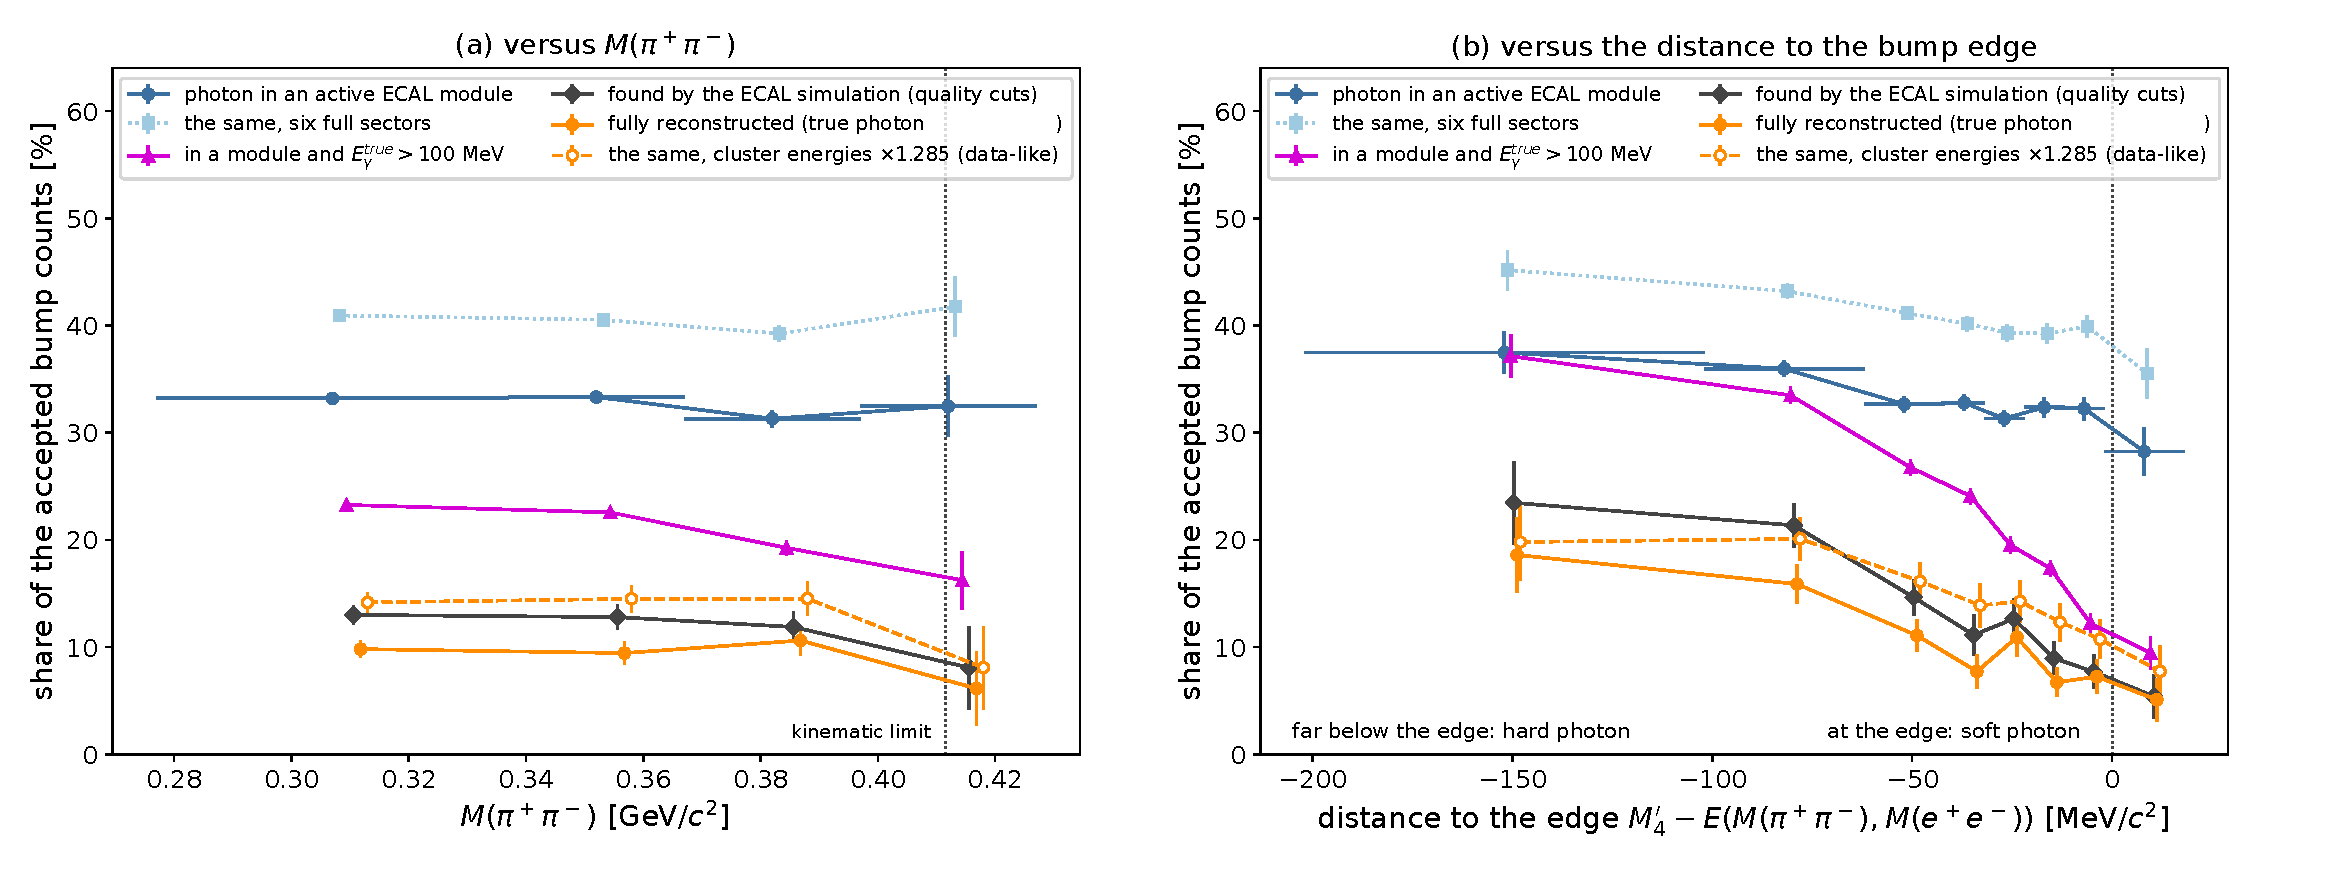
\includegraphics[width=\textwidth]{figs_all/ecalacc_fractions_cnt_short.pdf}
\caption{\textbf{What it shows: one third of the lost bump photons hit an active ECAL module at every \Mpipi, but near
the edge the photon is too soft for the 100\,MeV threshold, so the full reconstruction sees preferentially the part of
the bump far below the edge.} Finding of Part~III (\code{report_all.pdf}); simulation only. Blue: photon in an active
module (light blue: the same if all six sectors worked; one is off); magenta: in a module and true energy above 100\,MeV; dark grey: found by the ECAL
simulation with the quality cuts; orange: fully reconstructed; open orange: the same with the simulated cluster energies
$\times1.285$ (the energy scale of the data). (a) Against \Mpipi (dotted: kinematic limit 0.4116\,\GeVcc); (b) against the
distance to the bump edge, $u$.
\sel \simonly; accepted counts of the two bump channels (\piz Dalitz pair or converted photon); \basesel; no further cut
(every bump count has \Mee below 135\,\MeVcc, so $u$ exists for all of them).
ECAL quality cuts: identified as a photon, velocity $0.8<\beta<1.2$, cluster energy above 100\,MeV. Fully reconstructed:
the photon of the analysis' ECAL tag is the true lost photon, and $M(\pipi\ee\gamma)$, with the photon energy rescaled so
that $M(\ee\gamma)$ is the \piz mass, lies in 0.49--0.62\,\GeVcc.
\infig $E_\gamma^{\mathrm{true}}$ = true photon energy; $M_4'-E(\ldots)$ = $u$, with the simulated \Mfour on the data mass
scale. Magenta and orange here are not the bump channels of Fig.~\ref{fig:res_edgeu}.}
\label{fig:res_ecal}
\end{figure}

\textbf{Found with Part~III: the ECAL and the lost photon of the bump} (Fig.~\ref{fig:res_ecal}). \emph{In short:}
one third of the lost bump photons hit an active ECAL module, but they are soft, so about one bump count in ten is fully
reconstructed in the simulation. The lost photon is not stored, but the four true charged momenta, $m_{\piz}$ and $m_\eta$
fix it up to one angle; this gives its direction and energy for every simulated bump count. Seen from the target centre the
ECAL covers 10.9--45.6$^\circ$; one ECAL sector (azimuth 63--117$^\circ$) is off and 8 modules are dead, as in the data, so
the active modules cover 8.45\,\% of $4\pi$. Of the lost photons 9.0\,\% fly below the ECAL band, 54.5\,\% into it and
36.5\,\% above it; $32.7\pm0.4$\,\% hit an active module, flat in \Mpipi. Half of all lost photons have less than 100\,MeV; inside the
modules the simulated ECAL finds a cluster for only about 65\,\% (not explained), and its cluster energy is 7--9\,\% low.
$9.8\pm0.6$\,\% of the bump counts are fully reconstructed (14.1\,\% at the energy scale of the data), preferentially far
below the edge; the tag is specific to the bump (12.7\,\% of its counts, against 0.8\,\% and 1.8\,\% of the two peak
channels). \emph{What it means:} a full reconstruction keeps about 10--14\,\% of the bump as a clean peak, but it needs the
photon energy scale, the module efficiency and at least ten times more simulated $\eta\to\pipi\piz$ before it can be a
measurement.

\begin{figure}[!htb]
\centering
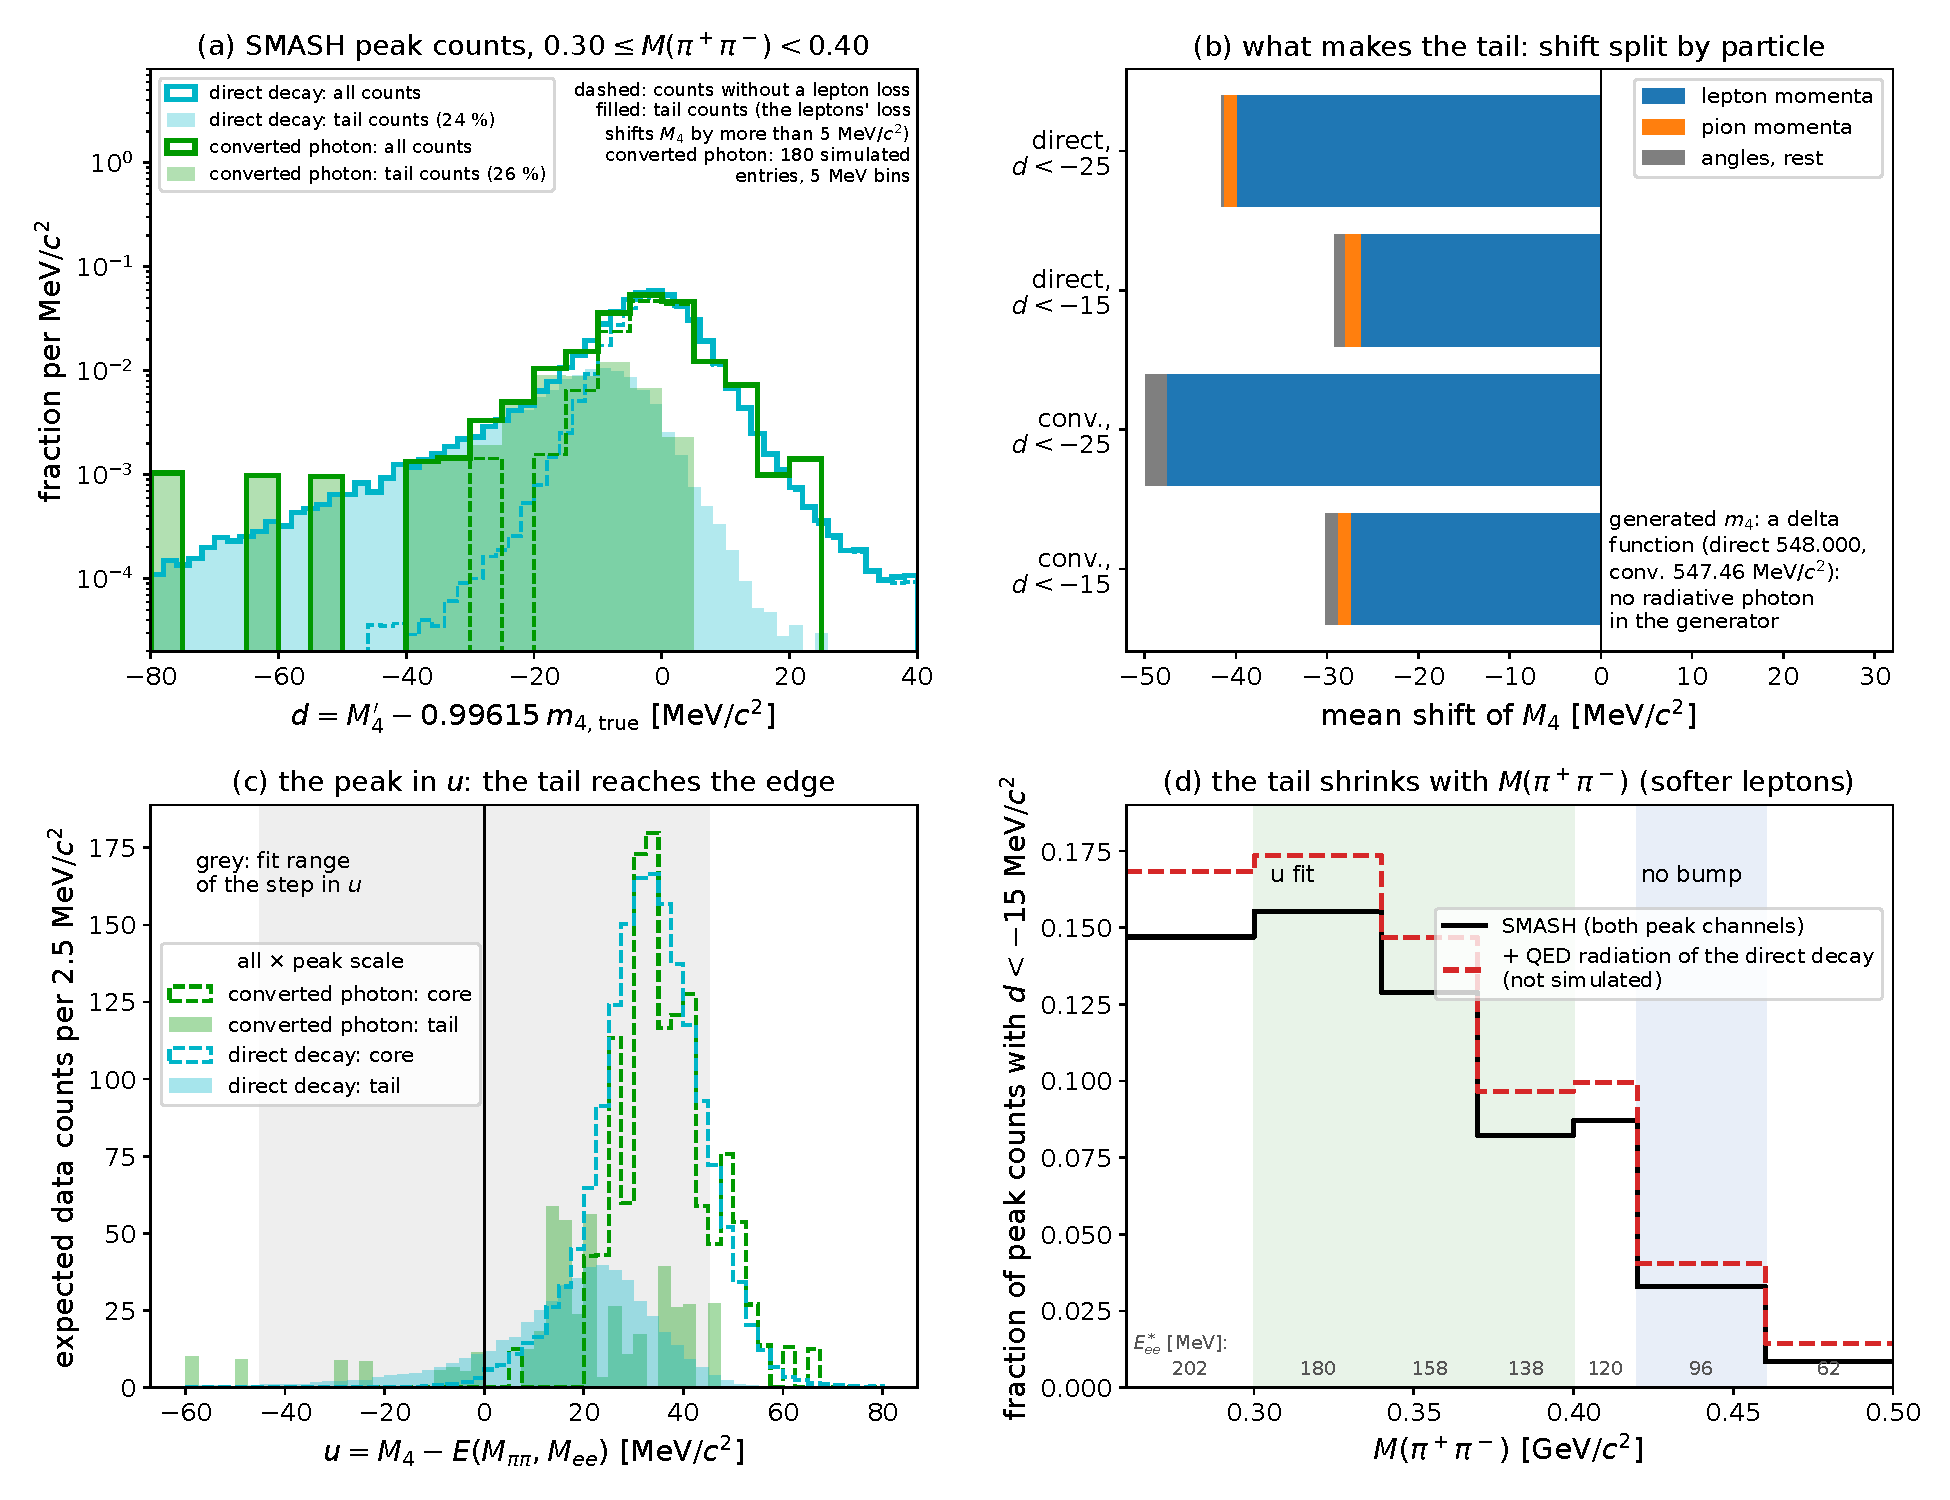
\includegraphics[width=0.72\textwidth]{figs_all/peaktail_sources_cnt_plain.pdf}
\caption{\textbf{What it shows: the tail of the simulated $\eta$ peak comes from the leptons' momentum loss in the material,
not from the generator; in $u$ it reaches the bump edge, and it shrinks at large \Mpipi.} Finding of Part~III
(\code{report_all.pdf}); simulation only. (a) Reconstructed minus generated \Mfour (generated value scaled by 0.99615) of the
peak counts: direct decay (cyan) and converted $\eta\to\pipi\gamma$ (green, 180 simulated entries in this selection); filled: tail counts (the
leptons' momentum loss lowers \Mfour by more than 5\,\MeVcc; 24 and 26\,\%); dashed: the other counts, symmetric. (b) Mean
shift of \Mfour for counts more than 15 or 25\,\MeVcc low, split into lepton momenta (blue), pion momenta (orange) and the
rest (grey). (c) The peak in $u$ (expected data counts, scaled by the peak scale 0.418 measured in Part~III): core dashed,
tail filled; grey: fit range of the step in $u$, $-45\le u<+45$\,\MeVcc. (d) Share of peak counts more than 15\,\MeVcc low per
\Mpipi bin: SMASH (black) and with the radiation of the direct decay that the generator lacks (red dashed, leading log); green
band ``u fit'': the \Mpipi range 0.30--0.40\,\GeVcc of the step fit in $u$; blue band ``no bump'': 0.42--0.46\,\GeVcc, above the
kinematic limit of the bump (0.4116\,\GeVcc).
\sel \simonly; the two peak channels; \basesel; both pion tracks used in the event-vertex fit; simulated masses on the data
mass scale ($\Mfour\times0.99615$, $\Mpipi\times0.9952$); $0.30\le\Mpipi<0.40$\,\GeVcc in (a)--(c), per \Mpipi bin in (d);
in (c) only \Mee below 135\,\MeVcc, where $u$ exists.
\infig $d = M_4'-0.99615\,m_{4,\mathrm{true}}$ = reconstructed minus true \Mfour on the data mass scale; all $\times$ peak scale
= scaled by the peak scale 0.418; $E^*_{ee}$ = \ee energy in the $\eta$ rest frame (upper axis of (d)).}
\label{fig:res_peaktail}
\end{figure}

\textbf{Found with Part~III: the tail of the simulated $\eta$ peak} (Fig.~\ref{fig:res_peaktail}). \emph{In short:}
the tail is made by the leptons, which lose momentum in the detector material (bremsstrahlung, HGeant); the generator writes
no radiative photon (the generated four-body mass is a sharp line), so the radiation of the decay itself is missing (it would
make the tail of the direct decay 16--19\,\% larger). About a quarter of the peak counts lose more than 5\,\MeVcc; in $u$,
5\,\% of the peak lies within 10\,\MeVcc of the edge, so the step fit of Part~III depends on the shape of the tail. The data
cannot measure its size; Part~III keeps the simulated tail and takes half of it as a systematic uncertainty (tail scale
$1\pm0.5$): $\pm3.4$\,\% on the bump scale from the edge in $u$, $\pm8.8$\,\% on the $\eta$ cross section from the peak.

\bigskip
\noindent{\Large\bfseries How the results were obtained}\par\nopagebreak
\makeatletter\@nobreaktrue\makeatother% no page break between this heading and the next section

%======================================================================
\section{Samples and normalisation}
\label{sec:samp}
\inshort{one SMASH run of $10^{10}$ p+p events, simulated three times (standard, lepton and $\eta$ sets), each set
worth $\Lsim = 221.05\,\nbinv$; one base selection.}
%======================================================================
\begin{itemize}
\item One SMASH run, p+p at $T = 4.5$\,GeV, $10^{10}$ events, impact parameter uniform in the area up to
      $b_{\max} = 1.2$\,fm. Each event stands for $\pi b_{\max}^2/N$, so every set has $\Lsim = 221.05\,\nbinv$.
\item Three sets of the \emph{same} events: \textbf{standard} (all decays natural), \textbf{lepton} (every \piz, $\eta$,
      $\rho^0$, $\omega$, $\phi$ forced into a dilepton channel), \textbf{$\eta$} (every $\eta$ forced: 50\,\%
      $\eta\to\ppee$, 50\,\% $\eta\to\pipi X17$). Each type of count is taken from one set only, with weights to the PDG
      branching ratios and the main physics weights of the $\eta$ decays (QED virtual-photon spectrum with form factors
      and decay angles for $\eta\to\ppee$, measured Dalitz plot for $\eta\to\pipi\piz$, pion form factor for
      $\eta\to\pipi\gamma$).
\item Chain: HGeant (detector simulation), reconstruction, the analysis program PAT (combinations of tracks, particle
      identification with cuts made for the simulation) and the final selection. The base selection: \basesel.
\item Trigger: PT3 is the main reaction trigger of the February 2022 beam time. It requires at least two of the six sectors with a hit
      in the inner TOF wall (iTOF) in coincidence with a hit in the outer TOF wall or in the RPC of the same sector, and at least three
      iTOF paddles hit (P.~Tlusty, ``LVL1 trigger in Feb22 p+p 4.5\,GeV'', HADES internal presentation, 13 December 2024, with the
      definition slide of I.~Ciepa{\l}). In the data only the bit of the trigger that arrives first is written, and PT3 events carry
      bit 8192. In the simulation a PT3 event carries both trigger bits (the value $12288=8192+4096$), so the simulated events are
      selected by the test ``bit 8192 set''.
\end{itemize}

%======================================================================
\section{Channels, cross sections and expected counts}
\label{sec:ch}
\inshort{visible cross sections from 0.0713\,nb (X17 at $\mathrm{BR}=10^{-5}$) to 7.05\,nb (bump with a \piz Dalitz
pair), i.e.\ 430 to 42\,900 counts at \Ldata, on a physical background of 686\,nb.}
%======================================================================
All cross sections here are \emph{visible} cross sections of reconstructed counts after the base selection:
$\sigma_{\mathrm{vis}} = \sigma_{\mathrm{prod}}\times\mathrm{BR}\times\varepsilon$, with the production from the
SMASH model, the branching ratios from PDG and the acceptance times efficiency $\varepsilon$ from the HADES
simulation.

\begin{table}[!htb]
\centering
\caption{Signal channels. $\sigma_{\mathrm{prod}}(\eta) = 1.0665\pm0.0016$\,mb (SMASH: 0.0236 $\eta$ per collision; later,
Part~III uses 1.0694\,mb for the whole sample, so $\varepsilon$ of the first three rows is 0.28\,\% too high; branching ratios
of PDG 2020). $\varepsilon$: reconstructed counts after the base selection per produced decay. $\sigma_{\mathrm{vis}}$ with
the physical decay kinematics (QED and form factors for the direct decay, measured Dalitz plot of $\eta\to\pipi\piz$, pion
form factor for $\eta\to\pipi\gamma$). Counts: expected at $\Ldata$, all \Mfour. X17 for an illustrative
$\mathrm{BR}=10^{-5}$.}
\label{tab:ch}
\footnotesize
\setlength{\tabcolsep}{3.5pt}
\begin{tabular}{@{}l l l r r r@{}}
\toprule
 & Process & BR (PDG) & $\varepsilon$ [\%] & $\sigma_{\mathrm{vis}}$ [nb] & counts \\
\midrule
bump      & $\eta\to\pipi\piz$, $\piz\to\ee\gamma$                 & $0.2292\times0.01174$ & $0.245\pm0.007$ & $7.05\pm0.19$ & 42\,900 \\
bump      & $\eta\to\pipi\piz$, a \piz photon converted             & $0.2292\times0.98823$ & $0.00212\pm0.00007$ & $5.19\pm0.17$ & 31\,600 \\
peak      & $\eta\to\pipi\gamma$, photon converted                 & 0.0422 & $0.00275\pm0.00017$ & $1.24\pm0.08$ & 7\,500 \\
peak      & $\eta\to\ppee$ (direct)                                 & $2.68\times10^{-4}$ & $0.4944\pm0.0013$ & $1.4168\pm0.0034$ & 8\,600 \\
X17       & $\eta\to\pipi X17$, $X17\to\ee$                         & $10^{-5}$ (hyp.) & $0.6665\pm0.0010$ & 0.0713 & 430 \\
\midrule
\multicolumn{4}{@{}l}{physical background (true \ee pair from one source, any pions)} & 686 & $4.17\times10^{6}$ \\
\multicolumn{4}{@{}l}{\quad multi-pion (\piz Dalitz, conversion, vector-meson pairs): 94\,\% of the sum} & & \\
\multicolumn{4}{@{}l}{fake lepton / leptons from two sources (shown, not added)} & 125 / 12.5 & \\
\bottomrule
\end{tabular}
\end{table}

The simulated spectrum after the base selection (Fig.~\ref{fig:spec}) is dominated by the multi-pion background;
the $\eta$ structures sit on top of it. Conversions are 42\,\% of the simulated bump and almost half of the peak.

%======================================================================
\section{What was corrected}
\label{sec:corr}
\inshort{six groups of corrections of the simulation chain, by weights or in the code; one tension remains
(an \ee opening angle above $2^\circ$ keeps 0.697 of the simulated peak, 0.778 of the data peak), and a finding of
Part~III concerns the bump.}
%======================================================================
\begin{enumerate}
\item \textbf{Generator codes stored with too few digits.} The analysis program stores the generator code of each track
      as a single-precision number, so codes above $2^{24}$ are rounded; all values were mapped back unambiguously.
\item \textbf{Weights of the lepton set.} The weighting first prescribed for this set counted a Dalitz lepton paired with
      its own conversion lepton 83 times too low; the weight of a count is now the product over the distinct forced decays of
      its four tracks (a second forced decay needs a factor 0.0985).
\item \textbf{One set per type of count.} The sets agree where they overlap (counts without a forced $\eta$, $\eta$ set
      against standard set: $1.0056\pm0.0036$).
\item \textbf{HGeant $\eta$ decay table.} The $\eta$ decay table used by HGeant in the production sets
      $\mathrm{BR}(\eta\to\ee\gamma) = 6.0\,\%$ instead of 0.60\,\%. The weights use the exact HGeant values: bump $-1.7\,\%$,
      conversion peak $+3.9\,\%$.
\item \textbf{The $\eta\to\ppee$ generator.} The channel is defined without a virtual photon, so its \Mee is not QED
      (27\,\% of the produced pairs within 0.5\,\MeVcc of threshold, 4.7\,\% above 20\,\MeVcc against 28\,\% for Kroll--Wada with
      phase space only). Counts are reweighted to Kroll--Wada with form factors and decay angles (31.3\,\% of the produced pairs
      above 20\,\MeVcc, Fig.~\ref{fig:res_defects}); after reconstruction and the base selection 0.219 of the simulated peak
      lies above 20\,\MeVcc (0.046 before), in agreement with Part~II's $0.23\pm0.04\pm0.05$. An opening angle above $2^\circ$
      then keeps $0.697\pm0.015$ of the simulated peak (0.59 before; data $0.778\pm0.033$, Part~II $0.772\pm0.037$): 0.81 of the
      direct decay but only 0.57 of the conversion peak, whose reconstructed opening angle is about $1.6^\circ$ larger than the
      true one (median $2.2^\circ$ against $0.5^\circ$). The producers should define the channel through a dilepton.
\item \textbf{Bookkeeping.} Smaller defects (trigger bit of the simulation, repeated entries of merged files, grouping of
      entries into events, single-precision sums that lost 3.4\,\%) are corrected in the code.
\end{enumerate}

\notebox{\textbf{Found with Part~III (\code{report_all.pdf}, section ``Efficiencies and the QED check of the
bump simulation'').} HGeant decays the virtual photon of the \piz Dalitz decay isotropically, while QED, and PLUTO
in the lepton set, give $1+\cos^2\theta^*$. The simulated efficiency of the bump with a \piz Dalitz pair is
therefore too high: by 12--14\,\% for prompt \piz Dalitz pairs, which explains the lepton/standard closure
$0.891\pm0.003$, and by about 16\,\% for the bump (factor about 0.86 for the bump edge, 0.864 over all \Mfour, 0.876 for the
ECAL-tagged counts, from the QED angle weighted count by count in the full simulation, the lost photon reconstructed on
its circle; the pseudo-experiments, 0.88, had too many soft leptons). Not corrected in this summary; Part~III weights every
simulated count of this channel with the QED angle, and its bump scales are 0.426 (edge in $u$) and 0.423 (edge per \Mpipi
slice).}

%======================================================================
\section{Final selection}
\label{sec:sel}
\inshort{the frozen peak cuts gain 5\,\% in $F$ over the base selection and the bump needs no cut; the usual $\eta$ cuts
do not improve the windows in the simulation; expected X17 limit $1.9\times10^{-5}$.}
%======================================================================
The cuts were optimised on simulation truth with $F = S/\sqrt{S+B}$: an exhaustive scan of nine cut variables, the
selection with the fewest cuts within 5\,\% of the best $F$ on the full sample and on both halves, and a split-half check of
the optimisation bias (below 1\,\% for the chosen cuts).

\begin{table}[!htb]
\centering
\caption{Frozen selections, all on top of the base selection. $S$, $B$: signal and background counts in the window at
\Ldata. Pion-track cut: both pion tracks within 40\,mm of the event vertex along the beam ($z$ of each track at its closest
approach to the beam axis).}
\label{tab:sel}
\small
\setlength{\tabcolsep}{4pt}
\begin{tabularx}{\textwidth}{@{}>{\raggedright\arraybackslash}p{4.3cm} L r r c c@{}}
\toprule
Target & Cuts & $S$ & $B$ & purity & efficiency \\
\midrule
peak (direct + conversion), $0.5333\le\Mfour<0.5587$ & pion-track cut, missing mass of \ppee below 2.85\,\GeVcc & 12\,800 & 41\,800 & 0.23 & 0.93 \\
direct decay only, same window & pion-track cut & 7\,100 & 52\,500 & 0.12 & 0.96 \\
bump, $0.4576\le\Mfour<0.5255$ & none & 58\,900 & 89\,800 & 0.40 & 1 \\
X17, peak window & $15.5\le\Mee<24.5$\,\MeVcc, both pions used in the event-vertex fit & 212.7 at $10^{-5}$ & 5\,342 & & \\
\bottomrule
\end{tabularx}
\end{table}

\begin{itemize}
\item The optimum is flat: many selections are within a few per cent of the best $F$. The gain of the frozen
      peak cuts over the base selection is 5\,\% in $F$.
\item The usual $\eta$ cuts (\usualcuts) remove background \emph{outside} the windows but do not improve them; the
      opening-angle cut alone keeps 0.81 of the direct decay (it costs 19\,\%). In the data (Parts~II, III) they do not pay off
      either: the CB is small (CB$/N$ = 0.07--0.10 in the peak window), the opening-angle cut keeps 0.78 of the data peak and
      lowers the precision in every selection, and Part~III does not apply the cuts.
\item X17: expected 90\,\% CL limit $1.9\times10^{-5}$ (at \Ldata), set by the simulation statistics of the
      background; $5.7\times10^{-6}$ if the background were known exactly. In the data (Part~III), with the background from
      the side bands, the limit is 0.114 times $\mathrm{BR}(\eta\to\ppee)$, i.e.\ $3.16\times10^{-5}$ with the PDG 2026
      value\footnote{\label{fn:x17pdg}With the PDG 2020 value $(2.68\pm0.11)\times10^{-4}$, used when the limit procedure
      was fixed, the same limit reads $3.06\times10^{-5}$.}, expected $2.68\times10^{-5}$ (68\,\% band 1.54--4.92); 1.9 is not
      like-for-like (it assumed all the SMASH $\eta$, the data hold about 0.4, and used a counting window). In the $\eta$ peak
      band ($0.5325\le\Mfour<0.5575$\,\GeVcc on the data mass scale) two thirds of the simulated X17 pairs have an opening angle below $6^\circ$, because they are fast (median pair
      momentum 424\,MeV/$c$); inside the X17 window, which also requires $15.5\le\Mee<24.5$\,\MeVcc, such a cut keeps only 58\,\%
      of the X17, as of the direct decays there (57\,\%). Every usual cut acts on X17 as on the direct decays within 5\,\%.
\end{itemize}

%======================================================================
\section{Signal extraction compared with the truth}
\label{sec:ext}
\inshort{in this test the template fit and the calibrated Gaussian fit recover the peak within a few per cent and the side
band with the simulated shape the bump; linear side bands lose the peak; the common simulation error must be added. The
current verdict for the data (Part~III, with the template noise of a real analysis) is in the last column of
Table~\ref{tab:blind}.}
%======================================================================
The methods planned for the data were applied blind to pseudo-data: half of the simulated events gave the templates,
the other half 200 pseudo-data sets by Poisson resampling (and 1500 parametric ones for X17); the methods were fixed
before the true content was looked at. Fig.~\ref{fig:toy} shows one pseudo-data set with the fits,
Table~\ref{tab:blind} and Fig.~\ref{fig:bias} the result.

\begin{figure}[!htb]
\centering
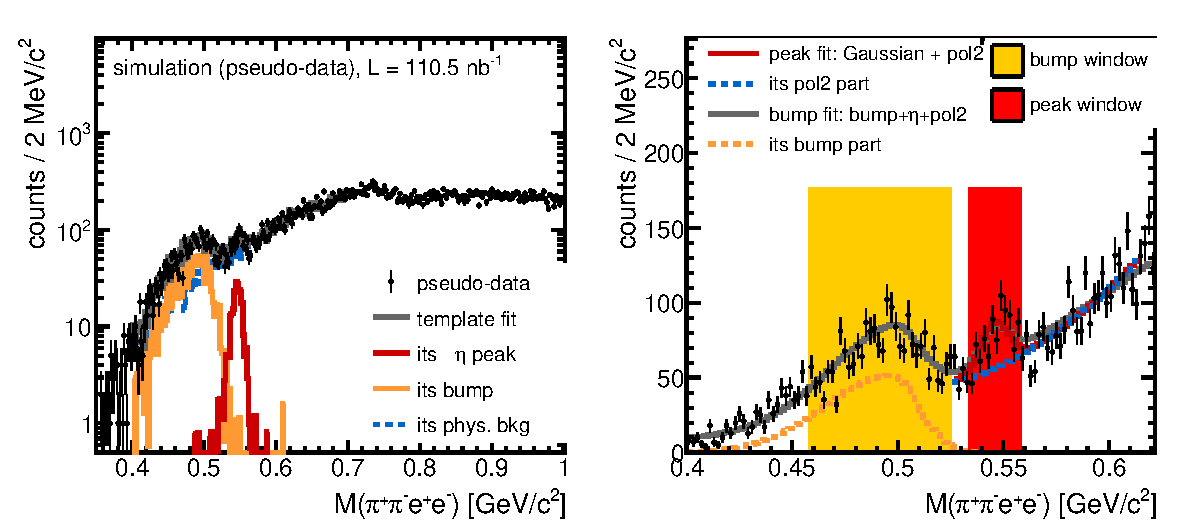
\includegraphics[width=0.84\textwidth]{figs/s5_blind_ana_toy0_PEAK_cnt_plain.pdf}
\caption{One pseudo-data set (110.5\,\nbinv). Left: \Mfour with the components of the template fit (fitted in
0.400--0.700\,\GeVcc). Right: zoom with the Gaussian + polynomial fit of the peak (0.526--0.614\,\GeVcc; its curve runs inside
the box of the peak window) and the parametric fit of the bump (0.400--0.620\,\GeVcc), with the bump and peak windows.
\sel \simonly; pseudo-data from one half of the simulated events, templates from the other; \basesel; both pion tracks
within 40\,mm of the event vertex along the beam; missing mass of \ppee below 2.85\,\GeVcc (frozen peak selection); \simwin.
\infig pol2 = second-order polynomial; its $\eta$ peak, its bump = both peak channels, both bump channels of the template
fit; phys.\ bkg = physical background.}
\label{fig:toy}
\end{figure}

\begin{figure}[!htb]
\centering
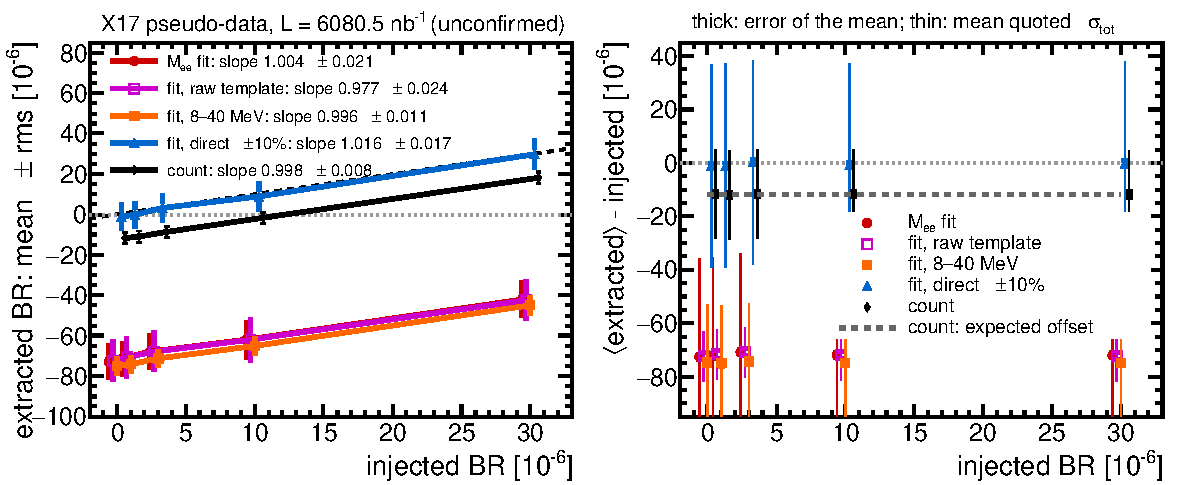
\includegraphics[width=0.84\textwidth]{figs/s5_blind_eval_x17_linearity_plain.pdf}
\caption{Blind test, X17: extracted against injected branching ratio (300 pseudo-data sets per point, 1500 in all, at
6080.5\,\nbinv) with straight-line fits, and the offset at zero. All estimators follow the injected value with slope
0.98--1.02. The zero point is shifted by the same amount in every pseudo-data set, because all of them share the same
unsmoothed simulated background (one simulated entry stands for about 55 expected data counts), which differs from the
template half: by $-72$ to $-75\times10^{-6}$ for the three fits with a free direct-decay normalisation, by $-11.7\times10^{-6}$
for counting (predicted from the difference of the two halves: $-11.76\times10^{-6}$), and by only $-1.1\times10^{-6}$ when the
direct-decay normalisation is constrained. A valid limit must therefore include the uncertainty of the background.
\sel \simonly; parametric pseudo-data around one half of the simulated events, templates and background from the other;
\basesel; both pion tracks used in the event-vertex fit; $13.0\le\Mee<26.5$\,\MeVcc and $0.5330\le\Mfour<0.5555$\,\GeVcc
(first version of the X17 selection, simulation mass scale).
\infig M$_{ee}$ fit = fit of the \Mee spectrum in the window with free normalisations of the direct decay and the rest; fit,
raw template = the same with the unsmoothed template; fit, 8--40\,MeV = the same on 8--40\,\MeVcc; fit, direct $\pm10$\,\% = the
same with the direct-decay normalisation constrained to $1\pm0.10$; count = counting with the background of the template half;
count: expected offset = the offset predicted for counting; $\sigma_{\mathrm{tot}}$ = quoted error.}
\label{fig:x17}
\end{figure}

\begin{table}[!htb]
\centering
\caption{Extracted yield against the truth, mean over 200 pseudo-data sets (frozen peak, direct-decay and bump selections).
The common uncertainty of the simulation templates ($\pm$11--15\,\% peak, $\pm$4.5--5\,\% bump) is shared by all methods.
Coverage: fraction of pseudo-data sets within the quoted error (nominal 0.68). Last column: the current verdict, from
Part~III's stress test with the template noise of a real analysis (Fig.~\ref{fig:stress}); the calibrated Gaussian was not
tested there.}
\label{tab:blind}
\small
\begin{tabularx}{\textwidth}{@{}>{\raggedright\arraybackslash}p{2.0cm} >{\raggedright\arraybackslash}p{3.9cm} r c L@{}}
\toprule
Yield & Method & bias & coverage & current verdict \\
\midrule
peak   & template fit                         & $+1.4\,\%$  & 0.77 & cross-check: $-6.6$\,\% with the template noise of a real analysis \\
       & Gaussian + polynomial, calibrated    & $+3.1\,\%$  & 0.72 & good here; not retested \\
       & linear side bands                    & $-21\,\%$   & 0.53 & loses signal as it stands; with the leak of the peak corrected and the background ratio from the smoothed simulation it is the peak measurement of Part~III ($-0.5$\,\%) \\
bump   & side band with simulated shape       & $+3.9\,\%$  & 0.66 & not determined in the data \\
       & edge step                            & $+1.3\,\%$  & 0.76 & the bump measurement of Part~III, in $u$ (closure within 2\,\%); here 16\,\% error \\
       & template fit / parametric fit        & $+7.7$ / $+5.4\,\%$ & 0.31 / 0.66 & somewhat high \\
direct decay alone & template fit, conversion constrained & $+20.6\,\%$ & 0.62 & limited by the conversion template \\
\bottomrule
\end{tabularx}
\end{table}

\textbf{What follows.}
\begin{itemize}
\item \textbf{Peak:} the template fit and the calibrated Gaussian fit reproduce the truth within a few per cent;
      in a single data set they may differ from each other by about 12\,\%. Linear side bands lose 13--46\,\% (about 30\,\%
      on average) because the background is convex under the peak. In Part~III the split of this test turned out to have four
      times the template noise of the real analysis; with realistic noise the template fits are pulled low (peak yield
      $-6.6$\,\%), because they scale a noisy signal template.
\item \textbf{Bump:} the side band with the simulated background shape is closest; the edge step is unbiased but
      imprecise. In Part~III the edge step, taken in $u$, is the bump measurement (closure within 2\,\% on 16\,000 pseudo-data
      sets); the side band with the simulated shape is not determined in the data, because its background has to be
      carried down 40--120\,\MeVcc.
\item \textbf{Direct decay alone:} \Mfour cannot separate it from the conversion peak; the split is limited by
      the 307 simulated entries of the conversion channel.
\item \textbf{X17:} the response is linear; a valid limit must include the uncertainty of the background,
      otherwise a background fluctuation can fake a signal (Fig.~\ref{fig:x17}).
\item The quoted errors describe the spread of the pseudo-data sets; the common simulation error must be added.
\end{itemize}

%======================================================================
\section{Open points}
\label{sec:open}
%======================================================================
\begin{itemize}
\item \textbf{Luminosity.} \Ldata is to be confirmed. It is the START-free elastic-scattering luminosity of all 17\,615 runs
      (Part~II), $\pm6.9$\,\%, liquid hydrogen only, still provisional; the 17\,557 analysed runs give 6079.2\,\nbinv, the value
      used in Parts~II and III.
\item \textbf{Simulation statistics.} The standard set limits the bump, conversion and X17-background templates: a larger
      production, and a forced $\eta\to\pipi\piz$ production ($\piz\to\ee\gamma$ and $\gamma\gamma$) with the full ECAL
      simulation, at least 10 times the present 2\,836 simulated bump entries, would reduce the dominant simulation error.
      In Part~III the template-statistics error is 1.6--3.6 times the statistical one.
\item \textbf{Producers:} confirm the HGeant $\eta\to\ee\gamma$ setting (6.0\,\%), regenerate the $\eta$ set with a
      dilepton definition of $\eta\to\ppee$, and match the simulated ECAL energy scale and resolution to the data after the
      new ECAL calibration.
\item \textbf{Beam energy:} the analysis uses $T = 4530$\,MeV, SMASH 4500\,MeV (affects the missing mass only). Part~III
      recomputes the simulated missing mass at 4500\,MeV; the effect on the cut at 2.85\,\GeVcc is about 0.3\,\%, and Part~II
      measures its efficiency in data as $0.972\pm0.023$ against 0.967 simulated.
\item \textbf{What the simulation lacks} (found with Parts~II and III). HGeant places the vertices only in the target
      segments: no collisions in the target walls or on the holder, no beam halo. The simulated vertex cut keeps 0.9997 of
      the direct decays. In the data 32\,\% of the \ee counts have no vertex (mostly not hydrogen events, probably from
      upstream of the cell; no measurable $\eta$: the vertex cut keeps $0.994\pm0.021$ of the $\eta$), and the empty-target runs show that the target walls give 13--15\,\% of
      the counts after CB subtraction in 0.40--0.70\,\GeVcc but only $3^{+4}_{-3}$\,\% of the $\eta$.
\item \textbf{Ghost-flagged pairs} (Part~III, not yet settled): a signal count with a ghost lepton stays signal, a
      true background pair with a ghost track counts as a fake lepton; moving the latter into the physical background raises
      the simulation by 9--17\,\% per region.
\item \textbf{PDG edition} (Part~III): the weights use PDG 2020; with PDG 2026 the direct decay would be
      $\times1.030$, the conversion peak $\times1.014$ and the bump $\times1.004$. The numbers here are kept; Part~III uses
      PDG 2026 everywhere, also for the X17 limit.
\item \textbf{ECAL efficiency} (Part~III): why does the simulated ECAL find a cluster for only about 65\,\% of the
      lost bump photons inside its active modules? About 4\,\% of the counts have a cluster from an $e^\pm$ of the converted
      photon instead; the rest is not explained.
\end{itemize}
The full report (\code{report_sim.pdf}, section ``Decisions awaiting the analyst's ruling'') lists the analysis decisions
behind these results; those still open (a larger simulation, requests to the simulation producers, an energy-loss cut against
electrons in the \pim slot) concern later work, and the numbers here are given without them.

\par\vspace{0pt plus 10\baselineskip}\penalty-300\vspace{0pt plus -10\baselineskip}% keep the table caption with its rows
{\footnotesize
\setlength{\tabcolsep}{4pt}
\renewcommand{\arraystretch}{1.08}
\begin{longtable}{@{}>{\raggedright\arraybackslash}p{3.3cm} >{\raggedright\arraybackslash}p{\dimexpr\textwidth-3.3cm-2\tabcolsep\relax}@{}}
\caption{\textbf{Notation} used in this summary. The full report defines every item in detail.}
\label{tab:nota}\\
\toprule
SMASH, PLUTO, HGeant, PAT & event generator; decay generator used to force decays; detector simulation of HADES; analysis program that builds the combinations of tracks and identifies the particles \\
\Lsim, \Ldata & integrated luminosity of one simulated set (221.05\,\nbinv); of the data (6080.5\,\nbinv, not confirmed) \\
count & one stored \pip\pim$e^+e^-$ combination of four tracks; an event can give more than one count \\
base selection & trigger, event vertex in the target region, particle identification, corrected momenta, all stored combinations; values in Sect.~\ref{sec:samp} \\
PT3 & the main reaction trigger: at least two sectors with an inner-TOF hit in coincidence with TOF or RPC, and at least three inner-TOF paddles hit (data: trigger bit 8192; simulation: bit 8192 set) \\
$\sigma_{\mathrm{prod}}$, BR, $\varepsilon$ & production cross section in SMASH; branching ratio (PDG unless stated); acceptance $\times$ efficiency: counts after the base selection per produced decay \\
$\sigma_{\mathrm{vis}}$ & visible cross section, $\sigma_{\mathrm{prod}}\times\mathrm{BR}\times\varepsilon$; counts at \Ldata $=\sigma_{\mathrm{vis}}\Ldata$ \\
bump, peak & $\eta\to\pipi\piz$ seen below $m_\eta$ (photon lost); $\eta$ seen at $m_\eta$ ($\eta\to\ppee$ or $\eta\to\pipi\gamma$ with conversion) \\
X17; target walls & hypothetical 17\,\MeVcc boson, $\mathrm{BR} = \mathrm{BR}(\eta\to\pipi X17)\,\mathrm{BR}(X17\to\ee)$; windows and wall of the hydrogen cell (not simulated, nor is the beam halo) \\
physical background; multi-pion & counts with a true \ee pair from one source and any pions; its part from \piz Dalitz, conversion and vector-meson pairs (no $\eta$) \\
fake lepton; two sources & a lepton slot holds a non-lepton or a ghost track; the two leptons come from different decays \\
CB & combinatorial background of the data (absent in simulation) \\
QED (Kroll--Wada), form factor & physical distribution of \Mee in a decay through a virtual photon; its hadronic modification \\
\Mfour, \Mee, \Mpipi & invariant mass of \ppee, of the \ee pair, of the \pipi pair \\
missing mass of \ppee & mass of (beam + target $-$ \pip\pim$e^+e^-$) four-momenta; for $pp\to pp\eta$ it is $M(pp)$ \\
opening angle; laboratory angle; $\eta$-rest angle & angle between $e^+$ and $e^-$; angle between the \pipi and \ee momenta in the laboratory; the same in the rest frame of a hypothetical $\eta$ with the measured \ppee momentum \\
pion-track cut; pions in the vertex fit & both pion tracks within 40\,mm of the event vertex along the beam; both pion tracks used in the fit of the event vertex \\
peak / bump window & $0.5333\le\Mfour<0.5587$ / $0.4576\le\Mfour<0.5255$\,\GeVcc (simulation mass scale) \\
$S$, $B$; purity, efficiency; $F$ & signal and other physical-background counts in a window at \Ldata; $S/(S+B)$, kept share of the signal of the base selection; $S/\sqrt{S+B}$ \\
pseudo-data set; bias; coverage & simulated data set from one half of the simulated events (the other half gives the templates); mean (extracted $-$ true); fraction of sets whose quoted error contains the truth (0.68 expected) \\
template noise & statistical fluctuation of the simulated templates; it pulls a fit that scales a noisy signal template towards zero \\
edge, $u$; edge step & the largest \Mfour of $\eta\to\pipi\piz$, $\piz\to\ee\gamma$ with the photon lost, at given \Mpipi and \Mee, $E(\Mpipi,\Mee)$; the distance to it, $u=\Mfour-E$ (for \Mee below 135\,\MeVcc); the height of the step of the spectrum there \\
ECAL; fully reconstructed & electromagnetic calorimeter (6 sectors of 163 modules; one sector, azimuth 63--117$^\circ$, off); a bump count whose lost photon is found in the ECAL and gives back the $\eta$ \\
\bottomrule
\end{longtable}
}

\end{document}
